\documentclass[aps,onecolumn,nofootinbib,pra]{article}

\usepackage{../../spec_files/arxiv}
\input{../../spec_files/standard_preamble.tex}

% Text Macros
\newcommand{\python}{$\mathrm{python}$}
\newcommand{\tnreason}{$\mathrm{tnreason}$}
\newcommand{\qcreason}{$\mathrm{qcreason}$}

\newcommand{\spengine}{$\mathrm{engine}$}
\newcommand{\sprepresentation}{$\mathrm{representation}$}
\newcommand{\spreasoning}{$\mathrm{reasoning}$}
\newcommand{\spapplication}{$\mathrm{application}$}

\newcommand{\layeronespec}{\textbf{Layer 1}: Storage and manipulations}
\newcommand{\layertwospec}{\textbf{Layer 2}: Specification of workload}
\newcommand{\layerthreespec}{\textbf{Layer 3}: Applications in reasoning}

% Current tnreason version
\newcommand{\curvertnreason}{2.0.0}

% Report Chapters
\newcommand{\partonetext}{Foundations} % was Classical Approaches
\newcommand{\chatextprobRepresentation}{Probability Distributions}
\newcommand{\chatextprobReasoning}{Probabilistic Inference}
\newcommand{\chatextlogicalRepresentation}{Propositional Logic}
\newcommand{\chatextlogicalReasoning}{Logical Inference}

\newcommand{\parttwotext}{Hybrid Logic Networks} % was Neuro-Symbolic Applications
\newcommand{\chatextformulaSelection}{Formula Selecting Networks}
\newcommand{\chatextnetworkRepresentation}{Hybrid Logic Representation}
\newcommand{\chatextnetworkReasoning}{Hybrid Logic Inference}
\newcommand{\chatextconcentration}{Probabilistic Guarantees}
\newcommand{\chatextfolModels}{First-Order Logic}

\newcommand{\partthreetext}{Contraction Calculus}
\newcommand{\chatextcoordinateCalculus}{Coordinate Calculus}
\newcommand{\chatextbasisCalculus}{Basis Calculus}
\newcommand{\chatextsparseCalculus}{Sparse Representation}
\newcommand{\chatextapproximation}{Sparse Optimization}
\newcommand{\chatextmessagePassing}{Message Passing}

\newcommand{\focusonespec}{Focus~I: Representation}
\newcommand{\focustwospec}{Focus~II: Reasoning}

% Sections in notation chapter and subsection in implementation.notation chapter, bn for basic notation
\newcommand{\bncategoricals}{Categorical Variables and Representations}
\newcommand{\bntensors}{Tensors}
\newcommand{\bncontractions}{Contractions}
\newcommand{\bnencoding}{Function encoding schemes}

%% Key Concepts of Part I

\newcommand{\probabilityTheory}{probability theory}
\newcommand{\ProbabilityTheory}{Probability theory}

\newcommand{\propositionalLogic}{propositional logic}
\newcommand{\PropositionalLogic}{Propositional logic}

% Decomposition mechanisms
\newcommand{\independenceMechanism}{independence mechanism}
\newcommand{\IndependenceMechanism}{Independence mechanism}
\newcommand{\computationMechanism}{computation mechanism}
\newcommand{\ComputationMechanism}{Computation mechanism}

\newcommand{\ComputationActivationNetwork}{Computation-Activation Network}
\newcommand{\ComputationActivationNetworks}{Computation-Activation Networks}

\newcommand{\CompActNet}{CompActNet}
\newcommand{\CompActNets}{CompActNets}

%% Key Concepts of Part II

% Networks
\newcommand{\MarkovLogicNetwork}{Markov Logic Network}
\newcommand{\HardLogicNetwork}{Hard Logic Network}
\newcommand{\HybridLogicNetwork}{Hybrid Logic Network}
\newcommand{\MarkovLogicNetworks}{Markov Logic Networks}
\newcommand{\HardLogicNetworks}{Hard Logic Networks}
\newcommand{\HybridLogicNetworks}{Hybrid Logic Networks}
\newcommand{\HybridFOLNetwork}{Hybrid First-Order Logic Network}
\newcommand{\HybridFOLNetworks}{Hybrid First-Order Logic Networks}

% Sparsity
\newcommand{\decompositionSparsity}{decomposition sparsity}
\newcommand{\DecompositionSparsity}{Decomposition sparsity}
\newcommand{\selectionSparsity}{selection sparsity}
\newcommand{\SelectionSparsity}{Selection sparsity}
\newcommand{\polynomialSparsity}{polynomial sparsity}
\newcommand{\PolynomialSparsity}{Polynomial sparsity}

% Tensor Structure
\newcommand{\substitutionStructure}{substitution structure}
\newcommand{\SubstitutionStructure}{Substitution structure}
\newcommand{\semanticStructure}{semantic structure}
\newcommand{\SemanticStructure}{Semantic structure}

\newcommand{\firstOrderLogic}{first-order logic}
\newcommand{\FirstOrderLogic}{First-order logic}


%% Key Concepts of Part III

% Encodings
\newcommand{\coordinateEncoding}{coordinate encoding}
\newcommand{\coordinateEncodings}{coordinate encodings}
\newcommand{\CoordinateEncoding}{Coordinate encoding}
\newcommand{\basisEncoding}{basis encoding}
\newcommand{\basisEncodings}{basis encodings}
\newcommand{\BasisEncoding}{Basis encoding}
\newcommand{\BasisEncodings}{Basis encodings}

% Calculus
\newcommand{\coordinateCalculus}{coordinate calculus}
\newcommand{\CoordinateCalculus}{Coordinate calculus}
\newcommand{\basisCalculus}{basis calculus}
\newcommand{\BasisCalculus}{Basis calculus}

% Sparse Representation
\newcommand{\basplusDecomposition}{basis+ $\cpformat$ decomposition}


%% Key Concepts of Quantum Circuit Extension
\newcommand{\ComputationActivationCircuit}{Computation Activation Circuit}
\newcommand{\ComputationActivationCircuits}{Computation Activation Circuits}

\newcommand{\computationCircuit}{computation circuit}
\newcommand{\computationCircuits}{computation circuits}
\newcommand{\ComputationCircuit}{Computation circuit}
\newcommand{\ComputationCircuits}{Computation circuits}

\newcommand{\activationCircuit}{activation circuit}
\newcommand{\activationCircuits}{activation circuits}
\newcommand{\ActivationCircuit}{Activation circuit}
\newcommand{\ActivationCircuits}{Activation circuits}

%% References

\newcommand{\defref}[1]{Def.~\ref{#1}}
\newcommand{\theref}[1]{Thm.~\ref{#1}}
\newcommand{\lemref}[1]{Lem.~\ref{#1}}
\newcommand{\corref}[1]{Cor.~\ref{#1}}
\newcommand{\algoref}[1]{Algorithm~\ref{#1}}
\newcommand{\probref}[1]{Problem~\eqref{#1}}
\newcommand{\exaref}[1]{Example~\ref{#1}}
\newcommand{\parref}[1]{Part~\ref{#1}}
\newcommand{\charef}[1]{Chapter~\ref{#1}}
\newcommand{\secref}[1]{Sect.~\ref{#1}}
\newcommand{\figref}[1]{Figure~\ref{#1}}
\newcommand{\assref}[1]{Assumption~\ref{#1}}
\newcommand{\remref}[1]{Remark~\ref{#1}}

\newcommand{\var}[1]{\text{\emph{#1}}}

\newcommand{\synencodingof}[1]{S\left(#1\right)} % Syntax encoding!
\newcommand{\stringof}[1]{\textit{"#1"}}

\newcommand{\rdf}{\mathrm{RDF}}
\newcommand{\mathrdftype}{\mathrm{rdf}\mathrm{type}}
\newcommand{\rdftype}{$\mathrm{rdf}:\mathrm{type}$}

\newcommand{\truesymbol}{\mathrm{True}}
\newcommand{\falsesymbol}{\mathrm{False}}
\newcommand{\truthset}{\{\falsesymbol,\truesymbol\}}
\newcommand{\truthstate}{z}
\newcommand{\truthstateof}[1]{\truthstate_{#1}}
\newcommand{\ozset}{\{0,1\}}
\newcommand{\ozbasisset}{\{\fbasisat{\catvariable},\tbasisat{\catvariable}\}}

\newcommand{\uniquantwrtof}[2]{\forall{#1}:{#2}}
\newcommand{\existquantwrtof}[2]{\exists{#1}:{#2}}
\newcommand{\imppremhead}[2]{\left(#1\right)\Rightarrow\left(#2\right)}

\newenvironment{centeredscript}% Use for tnreason script language, lstlistings for python code!
{\begin{center}
     \begin{algorithmic}
         \hspace{1cm}}
{\end{algorithmic}\end{center}}

\newcommand{\inlinecode}[1]{\lstinline[language=Python]|#1|}

\newcommand{\algdefsymbol}{\leftarrow}
\newcommand{\proofrightsymbol}{"$\Rightarrow$"}
\newcommand{\proofleftsymbol}{"$\Leftarrow$"}
\newcommand{\defcols}{\,:\,} % in definitions of functions
\newcommand{\wcols}{\,:\,} % in definitions of sets
\newcommand{\ncond}{,\,} %next cond
\newcommand{\defspace}{\quad,\quad}
\newcommand{\andspace}{\quad\text{and}\quad}
\newcommand{\ifspace}{\text{if}\quad}
\newcommand{\stspace}{\quad \text{subject to} \quad}

\newcommand{\iosepline}{\vspace{0.5em} \hrule \vspace{0.5em}}

\newcommand{\distassymbol}{\sim}
\newcommand{\probtagtypeinst}[2]{\mathrm{P}^{#1}_{#2}}

\newcommand{\mprojectionsymbol}{\mathrm{M}}
\newcommand{\iprojectionsymbol}{\mathrm{I}}
\newcommand{\gainsymbol}{\mathrm{gain}}
\newcommand{\gradientsymbol}{\mathrm{grad}}
\newcommand{\greedysymbol}{\mathrm{greedy}}
\newcommand{\hubosymbol}{\mathrm{HUBO}}
\newcommand{\maximizationsymbol}{\mathrm{max}}

% Entropies
\newcommand{\entropysymbol}{\mathbb{H}}
\newcommand{\sentropyof}[1]{\entropysymbol\left[#1\right]}
\newcommand{\sentropyofwrt}[2]{\entropysymbol_{#2}\left[#1\right]}
\newcommand{\centropyof}[2]{\entropysymbol\left[#1,#2\right]}
\newcommand{\centropyofwrt}[3]{\entropysymbol_{#3}\left[#1,#2\right]}
\newcommand{\kldivsymbol}{\mathrm{D}_{\mathrm{KL}}}
\newcommand{\kldivof}[2]{\kldivsymbol\left[ #1 || #2 \right]}
\newcommand{\mutinfof}[2]{I\left(#1;#2\right)}
\newcommand{\condmutinfof}[3]{\mutinfof{#1}{#2|#3}}
\newcommand{\subspacedimof}[1]{\mathrm{dim}(#1)}

\newcommand{\subsphere}{\mathbb{S}}
\newcommand{\rr}{\mathbb{R}}
\newcommand{\nn}{\mathbb{N}}

\newcommand{\closureof}[1]{\overline{#1}}
\newcommand{\interiorof}[1]{{#1}^{\circ}}
\newcommand{\sbinteriorof}[1]{{\left(#1\right)}^{\circ}}

\newcommand{\difofwrt}[2]{\frac{\partial #1}{\partial #2}}
\newcommand{\difwrt}[1]{\difofwrt{}{#1}}
\newcommand{\gradwrt}[1]{\nabla_{#1}}
\newcommand{\gradwrtat}[2]{\nabla_{#1}|_{#2}}

\newcommand{\cardof}[1]{\left|#1\right|}
\newcommand{\absof}[1]{\left|#1\right|}

\newcommand{\imageof}[1]{\mathrm{im}\left(#1\right)}

\newcommand{\convhullof}[1]{\mathrm{conv}\left(#1\right)}
\newcommand{\cubeof}[1]{[0,1]^{#1}}
\newcommand{\dimof}[1]{\mathrm{dim}\left(#1\right)}
\newcommand{\spanof}[1]{\mathrm{span}\left(#1\right)}
\newcommand{\subspaceof}[1]{V^{#1}}

\newcommand{\argmin}{\mathrm{argmin}}
\newcommand{\argmax}{\mathrm{argmax}}

% Help functions
\newcommand{\chainingfunction}{h}
\newcommand{\chainingfunctionof}[1]{\chainingfunction\left(#1\right)}

\newcommand{\greaterthanfunction}[1]{\ones_{>#1}}
\newcommand{\greaterthanfunctionof}[2]{\greaterthanfunction{#1}\left(#2\right)}
\newcommand{\existquanttrafo}{\greaterthanfunction{0}}
\newcommand{\universalquanttrafo}{\greaterthanfunction{\inddim-1}}

\newcommand{\greaterzerofunction}{\greaterthanfunction{0}}
\newcommand{\greaterzeroof}[1]{\greaterzerofunction\left(#1\right)}
\newcommand{\equalzeroof}[1]{\ones_{\{0\}}\left(#1\right)}
\newcommand{\equaloneof}[1]{\ones_{\{0\}}\left(#1\right)}

\newcommand{\nonzerofunction}{\ones_{\neq0}}
\newcommand{\nonzeroof}[1]{\nonzerofunction\left(#1\right)}
\newcommand{\nonzerocirc}{\nonzerofunction\circ}

\newcommand{\valof}[1]{\mathrm{val}\left(#1\right)}

% Probability distributions
\newcommand{\expof}[1]{\mathrm{exp}\left[#1\right]}
\newcommand{\probtensor}{\mathbb{P}}
\newcommand{\probtensorof}[1]{\probtensor^{#1}}
\newcommand{\probtensorofat}[2]{\probtensor^{#1}\left[#2\right]}
\newcommand{\secprobtensor}{\tilde{\mathbb{P}}}
\newcommand{\secprobat}[1]{\secprobtensor[#1]}
\newcommand{\secprobwith}{\secprobat{\shortcatvariables}}

\newcommand{\probfamilyofat}[3]{\probofat{#1}{#2|#3}}
\newcommand{\membervariable}{Z}
\newcommand{\memberindex}{z}
\newcommand{\indexedmembervariable}{\membervariable=\memberindex}
\newcommand{\probfamilywith}{\probfamilyof{}{\shortcatvariables}{\membervariable}}

\newcommand{\independent}[2]{\left(#1\perp#2\right)}
\newcommand{\condindependent}[3]{\left(#1\perp#2\middle)\,\right|\,#3}

\newcommand{\probtensorset}{\Gamma}
\newcommand{\probtensorin}{\probtensor\in\probtensorset}
\newcommand{\bmrealprobof}[1]{\realizabledistsof{\identity,\maxgraph,#1}}%
\newcommand{\alldists}{\realizabledistsof{\identity,\maxgraph}}

\newcommand{\gendistribution}{\probtensor^*}
\newcommand{\gendistributionat}[1]{\gendistribution\left[#1\right]}
\newcommand{\gendistributionwith}{\gendistributionat{\shortcatvariables}}
\newcommand{\currentdistribution}{\tilde{\probtensor}}
\newcommand{\currentdistributionat}[1]{\currentdistribution\left[#1\right]}
\newcommand{\currentdistributionwith}{\currentdistributionat{\shortcatvariables}}

\newcommand{\probat}[1]{\probtensor\left[#1\right]}
\newcommand{\probof}[1]{\probtensor^{#1}}
\newcommand{\probofat}[2]{\probof{#1}\left[#2\right]}
\newcommand{\probwith}{\probat{\shortcatvariables}}
\newcommand{\probwithnodes}{\probat{\nodevariables}}
\newcommand{\probofwrt}[2]{\probtensor_{#1}\left[#2\right]}

\newcommand{\condprobat}[2]{\mathbb{P}\big[#1\big|#2\big]}
\newcommand{\condprobof}[2]{\condprobat{#1}{#2}}
\newcommand{\condprobwrtof}[3]{\mathbb{P}^{#1}\big[#2\big|#3\big]}
\newcommand{\margprobat}[1]{\probat{#1}}
\newcommand{\expectationof}[1]{\mathbb{E}\left[#1\right]}
\newcommand{\expectationofwrt}[2]{\mathbb{E}_{#2}\left[#1\right]}
\newcommand{\lnof}[1]{\ln \left[ #1 \right] }
\newcommand{\sgnormof}[1]{\left\|#1\right\|_{\psi_2}} % subgaussian
\newcommand{\normof}[1]{\left\|#1\right\|_{2}}

\newcommand{\sinof}[1]{\mathrm{sin}\left(#1\right)}
\newcommand{\cosof}[1]{\mathrm{cos}\left(#1\right)}

\newcommand{\paulixsymbol}{\sigma_1}
\newcommand{\paulixat}[1]{\paulixsymbol\left[#1\right]}

\newcommand{\yrotationsymbol}{R_Y}
\newcommand{\yrotationofat}[2]{\yrotationsymbol\left({#1}\right)\left[#2\right]}

\newcommand{\ones}{\mathbb{I}}
\newcommand{\onesof}[1]{\ones^{#1}}
\newcommand{\onesat}[1]{\ones\left[#1\right]}
\newcommand{\onesofat}[2]{\onesof{#1}\left[#2\right]}
\newcommand{\oneswith}{\onesat{\shortcatvariables}}
\newcommand{\zeros}{0}
\newcommand{\zerosat}[1]{\zeros\left[#1\right]}
\newcommand{\identity}{\dirdelta}
\newcommand{\identityat}[1]{\identity\left[#1\right]}

\newcommand{\bernoulliof}[1]{B(#1)}

\newcommand{\deltaof}[1]{\delta_{#1}} % used in coordinate calculus proofs

\newcommand{\indicatorof}[1]{\ones_{#1}}
\newcommand{\indicatorofat}[2]{\ones_{#1}\left[#2\right]}

\newcommand{\exmatrix}{M}
\newcommand{\matrixat}[1]{\exmatrix[#1]}
\newcommand{\matrixofat}[2]{\exmatrix^{#1}\left[#2\right]}

\newcommand{\exvector}{V}
\newcommand{\vectorof}[1]{\exvector^{#1}}
\newcommand{\vectorat}[1]{\exvector[#1]}
\newcommand{\vectorofat}[2]{\exvector^{#1}[#2]}

\newcommand{\restrictionofto}[2]{{#1}|_{#2}}
\newcommand{\restrictionoftoat}[3]{\restrictionofto{#1}{#2}\left[#3\right]}

\newcommand{\idsymbol}{\mathrm{Id}} % ! Different to delta tensor in \identity
\newcommand{\idrestrictedto}[1]{\restrictionofto{\idsymbol}{#1}}

%% KNOWLEDGE GRAPH
\newcommand{\kg}{\mathrm{KG}|_{\worldindices}}
\newcommand{\kgat}[1]{\kg\left[#1\right]}
\newcommand{\kgreptensor}{\bencodingof{\kg}}

\newcommand{\exaunaryrelation}{C}
\newcommand{\exabinaryrelation}{R}

\newcommand{\kgtriple}[3]{\braket{#1,#2,#3}}
\newcommand{\exunarytriple}{\kgtriple{\provariable}{\mathrdftype}{\exaunaryrelation}}
\newcommand{\exbinarytriple}{\kgtriple{\provariableof{0}}{\exabinaryrelation}{\provariableof{1}}}

\newcommand{\atomcreator}{\psi}
\newcommand{\atomcreatorofat}[2]{\atomcreator_{#1}\left[#2\right]}
\newcommand{\provariable}{Z}
\newcommand{\provariableof}[1]{\provariable_{#1}}

\newcommand{\sparql}{\mathrm{SPARQL}}
\newcommand{\joinsymbol}{\mathrm{JOIN}}

\newcommand{\subsymbol}{s}
\newcommand{\predsymbol}{p}
\newcommand{\objsymbol}{o}

\newcommand{\sindvariable}{\indvariableof{\subsymbol}}
\newcommand{\pindvariable}{\indvariableof{\predsymbol}}
\newcommand{\oindvariable}{\indvariableof{\objsymbol}}

\newcommand{\invrdftypesymbol}{\mathrm{typ}}


% HLN Parametrization
\newcommand{\hardlegset}{A}
\newcommand{\hardparam}{(\hardlegset,\headindexof{\hardlegset})}
\newcommand{\hybridparam}{(\hardlegset,\headindexof{\hardlegset},\canparam)}
\newcommand{\hybridparamsetofdim}[1]{\mathcal{P}_{#1}}
\newcommand{\hybridparamset}{\hybridparamsetofdim{\seldim}}
\newcommand{\hybridparamin}{\hybridparam\in\hybridparamset}

\newcommand{\sechardlegset}{\tilde{\hardlegset}}
\newcommand{\sechybridparam}{(\sechardlegset,\secheadindexof{\sechardlegset},\seccanparam)}

\newcommand{\genhybridparam}{(\hardlegset^*,\headindexof{\hardlegset^*},\canparam^*)}

\newcommand{\hardlegsetto}[1]{\hardlegset^{#1}}
\newcommand{\hardlegindicesto}[1]{\headindexof{\hardlegset}^{#1}}
\newcommand{\hardparamto}[1]{(\hardlegsetto{#1},\headindexof{\hardlegsetto{#1}})}

\newcommand{\hlnparameters}{\hlnstat,\hybridparam}
\newcommand{\hlnat}[1]{\probofat{\hlnparameters}{#1}}
\newcommand{\hlnwith}{\hlnat{\shortcatvariables}}
 % Hard leg set to a given dimension

% Propositional Logics: New square bracket notation
\newcommand{\formula}{f}
\newcommand{\formulaof}[1]{\formula_{#1}}
\newcommand{\formulaat}[1]{\formula\left[#1\right]}
\newcommand{\formulaofat}[2]{\formulaof{#1}\left[#2\right]}
\newcommand{\formulain}{\formula\in\formulaset}
\newcommand{\formulawith}{\formulaat{\shortcatvariables}}

\newcommand{\hlnformulaof}[1]{\formula^{\hlnstat,(#1)}}
\newcommand{\hlnformulaparams}{\hardlegset,\headindexof{\hardlegset}}
\newcommand{\sechlnformulaparams}{\tilde{\hardlegset},\secheadindex_{\tilde{\hardlegset}}}
\newcommand{\hlnformula}{\hlnformulaof{\hlnformulaparams}} % mean parameter formula
\newcommand{\hlnformulaat}[1]{\hlnformula\left[#1\right]}
\newcommand{\hlnformulawith}{\hlnformulaat{\shortcatvariables}}
\newcommand{\vertexformula}{\hlnformulaof{[\seldim],\meanparam}}
\newcommand{\vertexformulaat}[1]{\vertexformula\left[#1\right]}

\newcommand{\hlnformulato}[1]{\hlnformulaof{\hardparamto{#1}}} % closest HLN to mean param


\newcommand{\formulavar}{\headvariableof{\formula}}
\newcommand{\formulacc}{\bencodingof{\formula}} % computation core
\newcommand{\formulaccwith}{\bencodingofat{\formula}{\formulavar,\shortcatvariables}}

\newcommand{\enumformula}{\formulaof{\selindex}}
\newcommand{\enumformulaat}[1]{\enumformula\left[#1\right]}
\newcommand{\enumformulawith}{\enumformulaat{\shortcatvariables}}

\newcommand{\enumformulacc}{\bencodingof{\enumformula}} % computation core
\newcommand{\enumformulaccwith}{\bencodingofat{\enumformula}{\headvariableof{\selindex},\shortcatvariables}}

\newcommand{\exformula}{\formula}
\newcommand{\exformulavar}{\headvariableof{\exformula}}
\newcommand{\exformulaat}[1]{\exformula\left[#1\right]}

\newcommand{\clausedim}{n}
\newcommand{\clausedimof}[1]{\clausedim_{#1}}
\newcommand{\clauseenumerator}{l}
\newcommand{\clauseenumeratorin}{\clauseenumerator\in[\clausedim]}

\newcommand{\formulazerocoordinates}{\shortcatindices\wcols\formulaat{\shortcatindices}=0}
\newcommand{\formulaonecoordinates}{\shortcatindices\wcols\formulaat{\shortcatindices}=1}

\newcommand{\secexformula}{h} % Since g is atom
\newcommand{\secexformulavar}{\headvariableof{\secexformula}}
\newcommand{\secexformulaat}[1]{\secexformula\left[#1\right]}

\newcommand{\exformulain}{\exformula\in\formulaset}
\newcommand{\exformulaof}[1]{\exformula\left(#1\right)}

\newcommand{\formulasuperset}{\mathcal{H}}

% First order Logics
\newcommand{\folexformula}{q}
\newcommand{\folexformulaat}[1]{\folexformula\left[#1\right]}
\newcommand{\folexformulawith}{\folexformulaat{\indvariableof{\folexformula},\worldvariables}}


 % When representing \folexformula as \importancequery \rightarrow \headfolexformula
\newcommand{\folformulaset}{\mathcal{Q}}
\newcommand{\folexformulain}{\folexformula\in\folformulaset}
\newcommand{\folexformulaof}[1]{\folexformula_{#1}}

\newcommand{\folformulastat}{\countquantifier\folformulaset}
\newcommand{\restfolformulaset}{\restrictionofto{\folformulaset}{\worlddomain}}

\newcommand{\enumfolformula}{\folexformulaof{\selindex}}
\newcommand{\enumfolformulaat}[1]{\enumfolformula\left[#1\right]}

\newcommand{\countquantifier}{\#}

\newcommand{\headfolformula}{h}
\newcommand{\headfolexformula}{\headfolformula}
\newcommand{\headfolformulaof}[1]{\headfolformula_{#1}}
\newcommand{\headfolformulaofat}[2]{\headfolformulaof{#1}\left[#2\right]}

\newcommand{\folpredicate}{g}
\newcommand{\folpredicateof}[1]{\folpredicate_{#1}}
\newcommand{\folpredicates}{\folpredicateof{0},\ldots,\folpredicateof{\folpredicateorder-1}}
\newcommand{\folpredicateenumerator}{\atomenumerator} % Due to PL being a special case
\newcommand{\folpredicateorder}{\atomorder}
\newcommand{\folpredicateofat}[2]{\folpredicateof{#1}\left[#2\right]}

\newcommand{\folfunction}{v}
\newcommand{\folfunctionof}[1]{\folfunction_{#1}}

\newcommand{\folterm}{v}

\newcommand{\worlddomain}{\arbset} % Snce enumerated
\newcommand{\exindividual}{a}
\newcommand{\secindividual}{b}
\newcommand{\exindividualof}[1]{\exindividual_{#1}}

\newcommand{\atombasemeasure}{\nu}

\newcommand{\individuals}{\exindividualof{\indindexof{0}},\ldots,\exindividualof{\indindexof{\individualorder-1}}}
\newcommand{\individualsof}[1]{\exindividualof{0}^{#1},\ldots,\exindividualof{\individualorder-1}^{#1}} % Do not use, index already in individuals


%% Redundant to individual variables
%\newcommand{\individualvariable}{\indvariable}
%\newcommand{\individualvariableof}[1]{\indvariableof{#1}}
%\newcommand{\individualvariables}{\indvariablelist}

%\newcommand{\individualorder}{\indorder}
%\newcommand{\individualenumerator}{\indenumerator}
%\newcommand{\individualenumeratorin}{\indenumeratorin}

\newcommand{\variableindex}{\indindex}
\newcommand{\variableindexof}[1]{\indindexof{#1}}
\newcommand{\variableenumerator}{\indenumerator}
\newcommand{\variableorder}{\indorder}
\newcommand{\variableenumeratorin}{\indenumeratorin}
\newcommand{\variableindices}{\indindexof{0}\ldots\indindexof{\indorder-1}}

\newcommand{\exconnective}{\circ}
\newcommand{\connectiveof}[1]{\exconnective_{#1}}
\newcommand{\connectiveofat}[2]{\connectiveof{#1}\left[#2\right]}

\newcommand{\folworldsymbol}{W}



%% CONFUSING: DO NOT USE!
\newcommand{\dataworldat}[1]{\worldindices[#1]}
\newcommand{\dataworldwith}{\dataworldat{\selvariable,\shortindvariables}}

\newcommand{\worldvariables}{\catvariableof{\folworldsymbol}}
\newcommand{\worldindices}{\catindexof{\folworldsymbol}}
\newcommand{\indexedworldvariables}{\indexedcatvariableof{\folworldsymbol}}
\newcommand{\worldindexset}{\left(\bigtimes_{\seccatenumeratorin}\bigtimes_{\indindexof{\seccatenumerator}\in[\inddim]^{\indorderof{\seccatenumerator}+1}}[2]\right)
\times\left(\bigtimes_{\atomenumeratorin}\bigtimes_{\indindexof{\atomenumerator}\in[\inddim]^{\indorderof{\atomenumerator}}}[2]\right)
}
\newcommand{\worldtensorspace}{\left(\bigotimes_{\seccatenumeratorin}\bigotimes_{\indindexof{\seccatenumerator}\in[\inddim]^{\indorderof{\seccatenumerator}+1}}\rr^2\right)
\otimes\left(\bigotimes_{\atomenumeratorin}\bigotimes_{\indindexof{\atomenumerator}\in[\inddim]^{\indorderof{\atomenumerator}}}\rr^2\right)
}

\newcommand{\groundingofatwrt}[3]{{#1}|_{#3} \left[#2\right]}
\newcommand{\groundingofwrt}[2]{{#1}|_{#2}}
\newcommand{\groundingofat}[2]{{#1}|_{\worldindices} \left[#2\right]}
\newcommand{\groundingof}[1]{{#1}|_{\worldindices}}
\newcommand{\kggroundingof}[1]{{#1}|_{\worldindices}}
\newcommand{\kggroundingofat}[2]{\kggroundingof{#1}\left[#2\right]}

%% For the TCalculus Theorem
\newcommand{\coordinatetrafo}{\chainingfunction}
\newcommand{\gentensor}{T}
\newcommand{\basisslices}{U}

% Parameters 
\newcommand{\candidatelist}{\mathcal{M}}
\newcommand{\candidatelistof}[1]{\candidatelist^{#1}}

% Data Extraction Spec
\newcommand{\impformula}{p}
\newcommand{\fixedimpformula}{\underline{\impformula}}
\newcommand{\fixedimpformulaat}[1]{\fixedimpformula\left[#1\right]}
\newcommand{\fixedimpformulawith}{\fixedimpformulaat{\indvariableof{\impformula}}}
\newcommand{\fixedimpbm}{\basemeasureofat{\fixedimpformula}{\worldvariables}}
\newcommand{\supportedworlds}{\worldindices \wcols \groundingofat{\impformula}{\shortindvariables} = \fixedimpformulawith}
\newcommand{\impformulaat}[1]{\impformula\left[#1\right]}

\newcommand{\sampleind}{\indindexof{[\indorder]}^\datindex}
%\newcommand{\decgroundedimpformula}{\groundingof{\impformula}^{\mathrm{enum}}}


\newcommand{\extformula}{g}
\newcommand{\extformulaof}[1]{\extformula_{#1}}
\newcommand{\extformulaofat}[2]{\extformulaof{#1}\left[#2\right]}
\newcommand{\extformulas}{\extformulaof{0},\ldots,\extformulaof{\atomorder-1}}
\newcommand{\shortextformulas}{\extformulaof{[\atomorder]}}

\newcommand{\extractionrelation}{\exrelation}

\newcommand{\variableset}{A} % Still used in monomial decomposition, NOT for object sets! -> Use \hardlegset instead!
\newcommand{\variablesetof}[1]{\variableset^{#1}}

\newcommand{\formulaset}{\mathcal{F}}
\newcommand{\formulasetof}[1]{\formulaset_{#1}}

\newcommand{\secformulaset}{\tilde{\formulaset}}

\newcommand{\hardformulaset}{\kb}
\newcommand{\hfbasemeasure}{\basemeasureof{\hardformulaset}}
\newcommand{\hfbasemeasureat}[1]{\hfbasemeasure\left[#1\right]}
\newcommand{\softformulaset}{\formulaset}


% Formula Selecting
\newcommand{\larchitecture}{\mathcal{A}}
\newcommand{\larchitectureat}[1]{\larchitecture\left[#1\right]}

\newcommand{\inneuronset}{\mathcal{A}^{\mathrm{in}}}
\newcommand{\outneuronset}{\mathcal{A}^{\mathrm{out}}}

\newcommand{\lneuron}{\mathcal{N}}
\newcommand{\lneuronof}[1]{\lneuron_{#1}}
\newcommand{\lneuronat}[1]{\lneuron\left(#1\right)}
\newcommand{\lneuractivation}{\sencodingof{\lneuron}}
\newcommand{\lneuractivationat}[1]{\lneuractivation\left[#1\right]}

\newcommand{\fsnn}{\sencodingof{\larchitecture}}
\newcommand{\fsnnat}[1]{\fsnn\left[#1\right]}

\newcommand{\sliceselectionmapof}[1]{\sencodingof{\fselectionmapof{\land,#1}}}
\newcommand{\sliceselectionmapofat}[2]{\sliceselectionmapof{#1}\left[#2\right]}
\newcommand{\sliceselectionmapat}[1]{\sliceselectionmapofat{\catorder,\sliceorder}{#1}}

\newcommand{\skeleton}{S}
\newcommand{\skeletonof}[1]{\skeleton\left(#1\right)}
\newcommand{\skeletontensor}{\bencodingof{\skeleton}} %OLD! Use skeleton

\newcommand{\skeletoncore}{S}
\newcommand{\skeletoncoreof}[1]{\skeletoncore^{#1}}

\newcommand{\cselectionsymbol}{C}
\newcommand{\vselectionsymbol}{V}
\newcommand{\sselectionsymbol}{S}

\newcommand{\selinputvariable}{\selvariable}
\newcommand{\cselinputvariable}{\selvariableof{\cselectionsymbol}}
\newcommand{\vselinputvariable}{\selvariableof{\vselectionsymbol}}

\newcommand{\fselectionmap}{\hlnstat}
\newcommand{\fselectionmapof}[1]{\fselectionmap_{#1}}
\newcommand{\fselectionmapat}[1]{\fselectionmap\left(#1\right)}
\newcommand{\fselectionmapofat}[2]{\fselectionmap_{#1}\left(#2\right)}

\newcommand{\sencfselectionmap}{\sencodingof{\fselectionmap}}
\newcommand{\sencfselectionmapat}[1]{\sencfselectionmap\left[#1\right]}

\newcommand{\cselectionmap}{\fselectionmapof{\cselectionsymbol}}
\newcommand{\cselectionmapat}[1]{\fselectionmapofat{\cselectionsymbol}{#1}}

\newcommand{\senccselectionmap}{\sencodingof{\cselectionmap}}
\newcommand{\senccselectionmapat}[1]{\senccselectionmap\left[#1\right]}

\newcommand{\vselectionmap}{\fselectionmapof{\vselectionsymbol}}
\newcommand{\vselectionmapat}[1]{\fselectionmapofat{\vselectionsymbol}{#1}}
\newcommand{\vselectionheadvar}{\headvariableof{\vselectionsymbol}} % Replacing \catvariableof{\vselectionmap}

\newcommand{\sencvselectionmap}{\sencodingof{\vselectionmap}}
\newcommand{\sencvselectionmapat}[1]{\sencvselectionmap\left[#1\right]}

\newcommand{\sselectionmap}{\fselectionmapof{\sselectionsymbol}}
\newcommand{\sselectionmapat}[1]{\fselectionmapofat{\sselectionsymbol}{#1}}

\newcommand{\sencsselectionmapat}[1]{\sencodingofat{\fselectionmapof{\sselectionsymbol}}{#1}}

\newcommand{\vselectionmapof}[1]{\fselectionmapof{\vselectionsymbol,#1}} % tb deleted!

\newcommand{\tranfselectionmap}{\fselectionmap^T}

% Output variables - Following the catvariable convention
\newcommand{\seloutputvariable}{\catvariable}
\newcommand{\cseloutputvariable}{\catvariableof{\cselectionsymbol}}
\newcommand{\vseloutputvariable}{\headvariableof{\vselectionsymbol}}

% Tensor Core Representation
\newcommand{\selectorcore}{{\bsencodingof{\vselectionsymbol}}}
\newcommand{\selectorcoreof}[1]{\bsencodingof{\vselectionmapof{#1}}}

\newcommand{\selectorcomponentof}[1]{\hypercoreof{{#1}}} % Since not an basis encoding!
\newcommand{\selectorcomponentofat}[2]{\selectorcomponentof{#1}\left[#2\right]}

\newcommand{\parspace}{\rr^{\seldim}}
\newcommand{\fullparcube}{[0,1]^{\seldim}}
\newcommand{\boundaryparcube}{\{0,1\}^{\seldim}} % ! This is not the boundary of the cube
\newcommand{\parcubevertices}{\{0,1\}^{\seldim}}
\newcommand{\cubeface}{Q}

\newcommand{\cubefaceparam}{\variableset,\headindexof{\variableset}}

\newcommand{\unitvectoratof}[2]{e^{(#1)}_{#2}}
\newcommand{\parametrizingunittensor}{e_{\atomindices}} % Not required?

\newcommand{\placeholder}{Z} %% When not used in formulas, take the set for it
\newcommand{\placeholderof}[1]{\placeholder^{#1}}

\newcommand{\atomicformula}{\exformula}%{\catvariable}
\newcommand{\atomicformulaof}[1]{\atomicformula^{#1}}
\newcommand{\atomicformulaofat}[2]{\atomicformulaof{#1}\left[#2\right]}

\newcommand{\atomicformulas}{\catvariableof{[\atomorder]}} %{\{\atomicformulaof{\atomenumerator} :  \atomenumeratorin \}}
\newcommand{\enumeratedatoms}{\atomicformulaof{0},\ldots,\atomicformulaof{\atomorder-1}}
\newcommand{\atomformulaset}{\formulasetof{\mlnatomsymbol}}

\newcommand{\clause}{Z^{\lor}}
\newcommand{\clauseof}[2]{\clause_{#1,#2}}
\newcommand{\clauseofat}[3]{\clauseof{#1}{#2}\left[#3\right]}
\newcommand{\maxtermof}[1]{\clause_{#1}}
\newcommand{\maxtermformulaset}{\formulasetof{\mlnmaxtermsymbol}}

\newcommand{\term}{Z^{\land}}
\newcommand{\termof}[2]{\term_{#1,#2}}
\newcommand{\termofat}[3]{\termof{#1}{#2}\left[#3\right]}
\newcommand{\mintermof}[1]{\term_{#1}}
\newcommand{\mintermofat}[2]{\mintermof{#1}\left[#2\right]}
\newcommand{\mintermformulaset}{\formulasetof{\mlnmintermsymbol}}

\newcommand{\indexedplaceholderof}[1]{\placeholderof{#1}_{\atomlegindexof{#1}}}
\newcommand{\indexedplaceholders}{\indexedplaceholderof{1},\ldots,\indexedplaceholderof{\atomorder}}

\newcommand{\atomorder}{d}
\newcommand{\secatomorder}{r}
\newcommand{\atomenumerator}{k}
\newcommand{\secatomenumerator}{l}

\newcommand{\atomenumeratorin}{\atomenumerator\in[\atomorder]}
\newcommand{\secatomenumeratorin}{\secatomenumerator\in[\secatomorder]}
\newcommand{\atomlegindex}{\catindex}
\newcommand{\tatomlegindex}{\tilde{\atomlegindex}}
\newcommand{\atomlegindexof}[1]{\atomlegindex_{#1}}
\newcommand{\tatomlegindexof}[1]{\tatomlegindex_{#1}}
\newcommand{\atomindices}{{\atomlegindexof{0},\ldots,\atomlegindexof{\atomorder-1}}}
\newcommand{\atomindicesin}{\atomindices\in\atomstates}

%% OPTIMIZATION
\newcommand{\targettensor}{\energytensor}
\newcommand{\importancetensor}{I}

%% MARKOV LOGIC NETWORK
\newcommand{\loss}{\mathcal{L}_{\datamap}}
\newcommand{\lossof}[1]{\loss\left(#1\right)}
\newcommand{\mlnformulaset}{\mathcal{F}}
\newcommand{\mlnformulain}{\exformula\in\mlnformulaset}
\newcommand{\weight}{\theta}
\newcommand{\weightof}[1]{\weight_{#1}}
\newcommand{\weightat}[1]{\weight[#1]}

\newcommand{\mlnparameters}{\formulaset,\canparam}
\newcommand{\mlntrueparameters}{(\formulaset^*,\weight^*)}



% Examples
\newcommand{\mlnatomsymbol}{[\catorder]}
\newcommand{\mlnmintermsymbol}{\land}
\newcommand{\mlnmaxtermsymbol}{\lor}

\newcommand{\partitionfunction}{\mathcal{Z}}
\newcommand{\secpartitionfunction}{\tilde{\mathcal{Z}}}
\newcommand{\partitionfunctionof}[1]{\partitionfunction\left(#1\right)}
\newcommand{\secpartitionfunctionof}[1]{\secpartitionfunction\left(#1\right)}

\newcommand{\mlnprob}{\probtensorof{\mlnparameters}}
\newcommand{\mlnprobat}[1]{\expdistofat{\mlnparameters}{#1}}
\newcommand{\mlnenergy}{\energytensorof{\mlnparameters}}

\newcommand{\folmlnparameters}{\folformulastat,\canparam,\basemeasureof{\fixedimpformula}}
\newcommand{\folhlnparameters}{\folformulastat,\hybridparam}
% For Probabilistic Analysis



\newcommand{\mintermnoise}{\noiseof{\identity}}
\newcommand{\mlnnoise}{\noiseof{\hlnstat}}
\newcommand{\mlnnoiseat}[1]{\mlnnoise\left[#1\right]}

\newcommand{\fprob}{p} % Drop! This is mean parameter
\newcommand{\fprobof}[1]{\fprob^{(#1)}}

\newcommand{\bidistof}[1]{B\left(#1\right)}
\newcommand{\multidistof}[1]{\underline{B}\left(#1\right)}
\newcommand{\widthwrtof}[2]{\Omega_{#1}\left(#2\right)}
\newcommand{\widthatof}[2]{\widthwrtof{#1}{#2}}

\newcommand{\selbasisshort}{\Gamma}
\newcommand{\selbasislong}{\{\onehotmapofat{\selindex}{\selvariable} \,:\, \selindexin \}}

\newcommand{\failprob}{u}
\newcommand{\precision}{t}
\newcommand{\maxgap}{\Delta}
\newcommand{\maxgapofat}[2]{\maxgap_{#1}\left(#2\right)}
\newcommand{\maxgapof}[1]{\maxgap\left(#1\right)}

%% CONTRACTION 
\newcommand{\invtemp}{\beta}

%% Hard Logic
\newcommand{\kb}{\mathcal{KB}}
\newcommand{\kbvar}{\headvariableof{\kb}}
\newcommand{\kbat}[1]{\kb\left[#1\right]}
\newcommand{\kbwith}{\kbat{\shortcatvariables}}

\newcommand{\seckb}{\tilde{\kb}}

%% Tensor Network Formats
\newcommand{\elformat}{\mathrm{EL}}
\newcommand{\cpformat}{\mathrm{CP}}
\newcommand{\htformat}{\mathrm{HT}}
\newcommand{\ttformat}{\mathrm{TT}}
\newcommand{\maxformat}{\mathrm{MAX}}

\newcommand{\elgraph}{\elformat}%{\graphof{\elformat}}
\newcommand{\maxgraph}{\maxformat}%{\graphof{\maxformat}}

\newcommand{\tnset}{\mathcal{T}}
\newcommand{\tnsetof}[1]{\tnset^{#1}} % of hypergraph
\newcommand{\eltnset}{\tnsetof{\elgraph}}

\newcommand{\objof}[1]{O\left(#1\right)} % Objective of optimization

\newcommand{\nodevariables}{\catvariableof{\nodes}}
\newcommand{\nodevariablesof}[1]{\catvariableof{\nodesof{#1}}}
\newcommand{\indexednodevariables}{\indexedcatvariableof{\nodes}}
\newcommand{\edgevariables}{\catvariableof{\edge}}
\newcommand{\extnetdist}{\normalizationof{\extnet}{\nodevariables}}

\newcommand{\secnodevariables}{\catvariableof{\secnodes}}

\newcommand{\extnetasset}{\left\{\hypercoreofat{\edge}{\catvariableof{\edge}}\wcols\edgein\right\}}

%% Probability Representation
\newcommand{\exrandom}{\catvariableof{0}}
\newcommand{\secexrandom}{\catvariableof{1}}
\newcommand{\thirdexrandom}{\catvariableof{2}}

\newcommand{\indexedexrandom}{\indexedcatvariableof{0}}
\newcommand{\indexedsecexrandom}{\indexedcatvariableof{1}}
\newcommand{\indexedthirdexrandom}{\thirdexrandom=\thirdexrandind}

\newcommand{\exrandind}{\catindexof{0}}
\newcommand{\exranddim}{\catdimof{0}}
\newcommand{\exrandindin}{\exrandind\in[\exranddim]}

\newcommand{\secexrandind}{\catindexof{1}}
\newcommand{\secexranddim}{\catdimof{1}}
\newcommand{\secexrandindin}{\secexrandind\in[\secexranddim]}

\newcommand{\thirdexrandind}{\catindexof{2}}
\newcommand{\thirdexranddim}{\catdimof{2}}
\newcommand{\thirdexrandindin}{\thirdexrandind\in[\thirdexranddim]}

% Hidden Markov Models
\newcommand{\randome}{E}
\newcommand{\randomeof}[1]{\randome_{#1}}
\newcommand{\tenumerator}{t}
\newcommand{\tdim}{T}
\newcommand{\tenumeratorin}{\tenumerator\in[\tdim]}

%% Exponential families
\newcommand{\expdistof}[1]{\probtensorof{#1}}
\newcommand{\expdistofat}[2]{\expdistof{#1}[#2]}
\newcommand{\expdist}{\probtensorof{(\sstat,\canparam,\basemeasure)}}
\newcommand{\expdistwith}{\probtensorofat{(\sstat,\canparam,\basemeasure)}{\shortcatvariables}}
\newcommand{\expdistat}[1]{\expdist\left[#1\right]}
\newcommand{\stanexpdistof}[1]{\expdistof{(\sstat,#1,\basemeasure)}}
\newcommand{\mlnexpdistof}[1]{\expdistof{(\formulaset,#1,\basemeasure)}}



\newcommand{\mnexpfamily}{\expfamilyof{\sstatof{\graph},\ones}} % The exponential family of Markov Networks on \graph
\newcommand{\mnexpfamilyof}[1]{\expfamilyof{\sstatof{#1},\ones}}
\newcommand{\mlnexpfamily}{\expfamilyof{\hlnstat,\ones}}

\newcommand{\stateset}{\mathcal{X}}
\newcommand{\sstatencoding}{\sencodingof{\sstat}}
\newcommand{\sstatencodingat}[1]{\sstatencoding\left(#1\right)}
\newcommand{\sstatencodingof}[1]{\gamma^{#1}}
\newcommand{\invsstatencodingat}[1]{\left(\sstatencoding\right)^{-1}\left(#1\right)}
\newcommand{\genstatshortcatencoding}[1]{\gamma^{\sstat}\left[\indexedshortcatvariables,\selvariable\right]}


\newcommand{\genfacemeasure}{\basemeasureof{\sstat,\facecondset}}
\newcommand{\genfacemeasureat}[1]{\basemeasureofat{\sstat,\facecondset}{#1}}
\newcommand{\genfacemeasurewith}{\genfacemeasureat{\shortcatvariables}}

\newcommand{\hlnfacemeasure}{\hlnformulaof{\facecondset}}
\newcommand{\hlnfacemeasureat}[1]{\hlnfacemeasure\left[#1\right]}
\newcommand{\hlnfacemeasurewith}{\hlnfacemeasureat{\shortcatvariables}}

\newcommand{\trivbm}{\ones}

\newcommand{\secbasemeasure}{\tilde{\basemeasure}}
\newcommand{\secbasemeasureat}[1]{\secbasemeasure\left[#1\right]}

\newcommand{\sstat}{t}%{\mathcal{S}}
\newcommand{\sstatat}[1]{\sstat\left(#1\right)}
\newcommand{\sstatof}[1]{\sstat^{#1}}
\newcommand{\secsstat}{\tilde{\sstat}}
\newcommand{\proposalstat}{\fselectionmap^T}

\newcommand{\hlnstat}{\sstat}%{\formulaset}
\newcommand{\hlnstatat}[1]{\sstatat{#1}}

\newcommand{\universalstat}{\identity}
\newcommand{\naivestat}{\universalstat}
\newcommand{\atomstat}{\shortcatvariables}

\newcommand{\sstatcoordinateof}[1]{\sstat_{#1}}
\newcommand{\sstatcoordinate}{\sstatcoordinateof{\selindex}}
\newcommand{\sstatcoordinateofat}[2]{\sstat_{#1}\left[#2\right]}

\newcommand{\sstatcc}{\bencodingof{\sstat}}
\newcommand{\sstatccwith}{\bencodingofat{\sstat}{\headvariables,\shortcatvariables}} % Same as \bencsstatwith

\newcommand{\hlnstatcc}{\bencodingof{\hlnstat}}
\newcommand{\hlnstatccwith}{\bencodingofat{\hlnstat}{\headvariables,\shortcatvariables}}

\newcommand{\sstatcatof}[1]{\headvariableof{#1}}

\newcommand{\sencsstat}{\sencodingof{\sstat}}
\newcommand{\sencsstatat}[1]{\sencodingof{\sstat}\left[#1\right]}
\newcommand{\sencsstatwith}{\sencsstatat{\shortcatvariables,\selvariable}}

\newcommand{\bencsstat}{\bencodingof{\sstat}}
\newcommand{\bencsstatat}[1]{\bencodingof{\sstat}\left[#1\right]}
\newcommand{\bencsstatwith}{\bencsstatat{\headvariables,\shortcatvariables}}

\newcommand{\sencfset}{\sencodingof{\formulaset}}
\newcommand{\sencfsetat}[1]{\sencfset\left[#1\right]}

\newcommand{\sencmlnstat}{\sencodingof{\hlnstat}}
\newcommand{\sencmlnstatat}[1]{\sencmlnstat\left[#1\right]}
\newcommand{\sencmlnstatwith}{\sencmlnstat\left[\shortcatvariables,\selvariable\right]}
\newcommand{\sencproposalstat}{\sencodingof{\proposalstat}}



\newcommand{\singlecanparam}{\canparam}

\newcommand{\seccanparam}{\tilde{\canparam}}
\newcommand{\seccanparamat}[1]{\seccanparam\left[#1\right]}

\newcommand{\canparamwrtat}[2]{\canparamofat{#1}{#2}}
\newcommand{\estcanparam}{\hat{\canparam}}
\newcommand{\naivecanparam}{\tilde{\canparam}}
\newcommand{\naivecanparamat}[1]{\naivecanparam\left[#1\right]}

\newcommand{\datacanparam}{\canparamof{\datamap}}
\newcommand{\datacanparamat}[1]{\canparamofat{\datamap}{#1}}

\newcommand{\gencanparam}{\canparamof{*}}
\newcommand{\gencanparamat}[1]{\canparamofat{*}{#1}}

\newcommand{\canmetric}{d}
\newcommand{\canmetricwrt}[1]{\canmetric_{#1}}
\newcommand{\canmetricwrtof}[3]{\canmetric_{#1}\left(#2,#3\right)}
\newcommand{\canmetricof}[2]{\canmetric\left(#1,#2\right)}


\newcommand{\canparamhypothesis}{\Gamma}
\newcommand{\canparamin}{\canparam\in\canparamhypothesis}

\newcommand{\greedyhypothesis}{\mathcal{H}}

\newcommand{\expsolution}{\gencanparam}
\newcommand{\empsolution}{\datacanparam}



\newcommand{\secmeanparam}{\tilde{\mu}}
\newcommand{\secmeanparamat}[1]{\secmeanparam\left[#1\right]}

\newcommand{\meanrepprob}{\probtensor^{\meanparam}}

\newcommand{\meanset}{\mathcal{M}}
\newcommand{\meansetof}[1]{\meanset_{#1}}
\newcommand{\genmeanset}{\meanset_{\sstat,\basemeasure}}
\newcommand{\hlnmeanset}{\meanset_{\hlnstat,\ones}}
\newcommand{\propmeanset}{\meanset_{\propstat,\ones}}

\newcommand{\elmeanset}{\meanset^{\elformat}}
\newcommand{\elmeansetof}[1]{\elmeanset_{#1}}
\newcommand{\elhlnmeanset}{\elmeansetof{\hlnstat,\basemeasure}}

\newcommand{\genmeansetargmax}{\argmax_{\meanparam\in\genmeanset}}
\newcommand{\cangenmeansetargmax}{\genmeansetargmax\contraction{\canparamwith,\meanparamwith}}
\newcommand{\cansstatcatindicesargmax}{\argmax_{\shortcatindices}\contraction{\canparam,\sstat(\shortcatindices)}}

\newcommand{\imset}{\mathcal{N}}
\newcommand{\imsetof}[2]{\imset_{#1}^{#2}}
\newcommand{\genimset}{\imsetof{\sstat,\basemeasure}{}}
\newcommand{\genfaceimset}{\imsetof{\sstat,\basemeasure}{\facesymbol}}

\newcommand{\imelement}{v}
\newcommand{\imelementof}[1]{\imelement^{#1}}
\newcommand{\imelementat}[1]{\imelement\left[#1\right]}
\newcommand{\imelementofat}[2]{\imelement^{#1}\left[#2\right]}
\newcommand{\imelementwith}{\imelementat{\selvariable}}

\newcommand{\normalvec}{a}
\newcommand{\normalbound}{b}
\newcommand{\normalvecofat}[2]{\normalvec_{#1}\left[#2\right]}
\newcommand{\normalboundof}[1]{\normalbound_{#1}}
\newcommand{\normalboundofat}[2]{\normalbound_{#1}\left[#2\right]}
\newcommand{\halfspaceparams}{\left( (\normalvecofat{i}{\selvariable},\normalboundof{i}) \wcols i \in[n]\right)}

\newcommand{\facesymbol}{\mathcal{F}} % Using the ziegler book notation
\newcommand{\facesymbolof}[1]{\facesymbol^{#1}}
\newcommand{\facelatticeof}[1]{L\left(#1\right)}
\newcommand{\genfacelattice}{\facelatticeof{\genmeanset}}
\newcommand{\facein}{\facesymbol\in\genfacelattice}

\newcommand{\facecondset}{\mathcal{I}} % OLD, Use instead \facesymbol
\newcommand{\facecondsetof}[1]{\facecondset^{#1}}
\newcommand{\faceset}{Q} % OLD, Use instead \facesymbol
\newcommand{\facesetofspec}[2]{\faceset^{#1}_{#2}}
\newcommand{\genfacesetof}[1]{\facesetofspec{#1}{\sstat,\basemeasure}}
\newcommand{\genfaceset}{\genfacesetof{\facecondset}}

\newcommand{\hlnfaceset}{\facesetofspec{\facecondset}{\hlnstat,\ones}}

\newcommand{\maxconeof}[1]{C^{#1}}
\newcommand{\maxcone}{\maxconeof{\facecondset}}

\newcommand{\genmaxconeof}[1]{C_{\sstat,\basemeasure}^{#1}}
\newcommand{\genmaxcone}{\genmaxconeof{\facecondset}}

\newcommand{\hlnmaxconeof}[1]{C_{\hlnstat,\basemeasure}^{#1}}
\newcommand{\hlnmaxcone}{\hlnmaxconeof{\facecondset}}

\newcommand{\datamean}{\meanparamof{\datamap}}
\newcommand{\datameanat}[1]{\datamean\left[#1\right]}
\newcommand{\datameanwith}{\datameanat{\selvariable}}

\newcommand{\genmean}{\meanparam^*}
\newcommand{\genmeanat}[1]{\genmean[#1]}
\newcommand{\genmeanwith}{\genmeanat{\selvariable}}

\newcommand{\currentmean}{\tilde{\meanparam}}
\newcommand{\currentmeanat}[1]{\currentmean\left[#1\right]}

\newcommand{\cumfunctionwrt}[1]{A^{#1}}
\newcommand{\cumfunctionwrtof}[2]{\cumfunctionwrt{#1}\left(#2\right)}
\newcommand{\cumfunction}{\cumfunctionwrt{(\sstat,\basemeasure)}}
\newcommand{\cumfunctionof}[1]{\cumfunction(#1)}
\newcommand{\dualcumfunction}{\big(\cumfunction\big)^*}
\newcommand{\dualcumfunctionof}[1]{\big(\cumfunction\big)^*(#1)}

\newcommand{\forwardmapwrt}[1]{F^{#1}}
\newcommand{\forwardmap}{\forwardmapwrt{(\sstat,\basemeasure)}}
\newcommand{\forwardmapwrtof}[2]{\forwardmapwrt{#1}(#2)}
\newcommand{\forwardmapof}[1]{\forwardmapwrtof{(\sstat,\basemeasure)}{#1}}
\newcommand{\forwardmapofat}[2]{\forwardmapof{#1}\left[#2\right]}

\newcommand{\backwardmapwrt}[1]{B^{#1}}
\newcommand{\backwardmap}{\backwardmapwrt{(\sstat,\basemeasure)}}
\newcommand{\backwardmapwrtof}[2]{\backwardmapwrt{#1}(#2)}
\newcommand{\backwardmapof}[1]{\backwardmapwrtof{(\sstat,\basemeasure)}{#1}}

\newcommand{\energyhypothesis}{\Theta}
\newcommand{\energyhypothesisof}[1]{\energyhypothesis^{#1}}

\newcommand{\graph}{\mathcal{G}}
\newcommand{\graphof}[1]{\graph^{#1}}
\newcommand{\secgraph}{\tilde{\graph}}
\newcommand{\nodes}{\mathcal{V}}
\newcommand{\nodesof}[1]{\nodes^{#1}}
\newcommand{\innodes}{\nodesof{\mathrm{in}}}
\newcommand{\outnodes}{\nodesof{\mathrm{out}}}

\newcommand{\domainsymbol}{k}
\newcommand{\domainedges}{\edgesof{\domainsymbol}}

\newcommand{\graphqueue}{\mathcal{Q}}



\newcommand{\prenodes}{\{\secnode \wcols \secnode \prec \node, \secnode\neq\node\}}
\newcommand{\afternodes}{\{\secnode \wcols \node \prec \secnode, \secnode\neq\node\}}

\newcommand{\incomingnodes}{\edge^{\mathrm{in}}}
\newcommand{\outgoingnodes}{\edge^{\mathrm{out}}}

\newcommand{\nodesa}{A}
\newcommand{\nodesb}{B}
\newcommand{\nodesc}{C}

\newcommand{\nodea}{a}
\newcommand{\nodeb}{b}

\newcommand{\nodesone}{\nodesof{1}}
\newcommand{\nodestwo}{\nodesof{2}}
\newcommand{\nodesthree}{\nodesof{3}}

\newcommand{\secnodes}{\mathcal{U}}%{\tilde{\nodes}}
\newcommand{\secnodesof}[1]{\tilde{\nodes}^{#1}}
\newcommand{\thirdnodes}{\mathcal{W}}%{\bar{\nodes}}

\newcommand{\node}{v}
\newcommand{\nodein}{\node\in\nodes}
\newcommand{\secnode}{\tilde{\node}}
\newcommand{\thirdnode}{\bar{\node}}

\newcommand{\edges}{\mathcal{E}}
\newcommand{\edgesof}[1]{\edges^{#1}}
\newcommand{\secedges}{\tilde{\edges}}

\newcommand{\edge}{e}
\newcommand{\edgeof}[1]{\edge_{#1}}
\newcommand{\secedge}{\tilde{\edge}}
\newcommand{\thirdedge}{\hat{\edge}}
\newcommand{\edgein}{\edge\in\edges}

\newcommand{\parentsof}[1]{\mathrm{Pa}(#1)}
\newcommand{\nondescendantsof}[1]{\mathrm{NonDes}(#1)}

\newcommand{\neighborsof}[1]{\mathrm{N}(#1)}

\newcommand{\bnnodecore}{\hypercoreof{(\parentsof{\node},\{\node\})}}
\newcommand{\bnedges}{\{(\parentsof{\node},\{\node\}) \wcols \nodein\}}

\newcommand{\hypercore}{\tau}
\newcommand{\hypercoreat}[1]{\hypercore\left[#1\right]}
\newcommand{\hypercorewith}{\hypercoreat{\shortcatvariables}}
\newcommand{\hypercorewithnodes}{\hypercoreat{\nodevariables}}
\newcommand{\hypercorewithin}{\hypercoreat{\shortcatvariables}\in\facspace}
\newcommand{\hyperonecoordinates}{\shortcatindices\wcols\hypercoreat{\indexedshortcatvariables} = 1}
\newcommand{\hyperzerocoordinates}{\shortcatindices\wcols\hypercoreat{\indexedshortcatvariables} = 0}

\newcommand{\edgehypercorewith}{\hypercoreofat{\edge}{\catvariableof{\edge}}}

\newcommand{\hypercoreof}[1]{\hypercore^{#1}}
\newcommand{\hypercoreofat}[2]{\hypercoreof{#1}\left[#2\right]}
\newcommand{\sechypercore}{\tilde{\hypercore}}
\newcommand{\sechypercoreof}[1]{\sechypercore^{#1}}
\newcommand{\sechypercoreofat}[2]{\sechypercore^{#1}\left[#2\right]}
\newcommand{\sechypercoreat}[1]{\sechypercore\left[#1\right]}

%% Factored System


\newcommand{\statevectorof}[1]{v_{#1}}
\newcommand{\statevectorofat}[2]{\statevectorof{#1}\left[#2\right]}

% Greedy
\newcommand{\extendedformulaset}{\formulaset\cup\{\formula\}}
\newcommand{\extendedcanparam}{\tilde{\canparam}\cup\{\weightof{\formula}\}}

\newcommand{\exfunction}{q}
\newcommand{\exfunctionof}[1]{\exfunction_{#1}}
\newcommand{\exfunctiontargetspace}{\bigotimes_{l\in[p]}\rr^{\catdimof{l}}}
\newcommand{\exfunctiontargetvariables}{Y_0,\ldots,Y_{p-1}}
\newcommand{\exfunctionimageelement}{y}
\newcommand{\exfunctionat}[1]{\exfunction(#1)}
\newcommand{\exfunctionofat}[2]{\exfunctionof{#1}(#2)}
\newcommand{\secexfunction}{g}
\newcommand{\secexfunctionat}[1]{\secexfunction(#1)}

\newcommand{\realvaluedfunction}{\exfunction}
\newcommand{\realvaluedfunctionev}[1]{\realvaluedfunction\left(#1\right)} % Evaluated
\newcommand{\realvaluedfunctionat}[1]{\realvaluedfunction\left[#1\right]}

\newcommand{\statesetfunction}{\exfunction}
\newcommand{\statesetfunctionev}[1]{\statesetfunction\left(#1\right)}

\newcommand{\tenvaluedfunction}{\exfunction}
\newcommand{\tenvaluedfunctionev}[1]{\tenvaluedfunction\left(#1\right)}
\newcommand{\tenvaluedfunctionat}[1]{\tenvaluedfunction\left[#1\right]}

\newcommand{\compositionof}[2]{{#1}\circ{#2}}
\newcommand{\compositionofat}[3]{(\compositionof{#1}{#2})(#3)}

%% Message Passing
\newcommand{\scheduler}{S}
\newcommand{\ovgraph}{\graph^{\mathrm{overlap}}} % overlap graph to the hypergraph
\newcommand{\dirovgraph}{\graph^{\rightarrow}} % directed overlap graph
\newcommand{\ovedges}{\edges^{\mathrm{overlap}}}
\newcommand{\dirovedges}{\edges^{\rightarrow}}

\newcommand{\sedge}{\edgeof{0}} % Send edge
\newcommand{\redge}{\edgeof{1}} % Receive edge
\newcommand{\secsedge}{\edgeof{2}}
\newcommand{\thirdsedge}{\edgeof{3}}

\newcommand{\preedgesetwrt}[2]{\edges^{\rightarrow(#1,#2)}}
\newcommand{\preedgeset}{\preedgesetwrt{\sedge}{\redge}}

\newcommand{\cluster}{C}
\newcommand{\clusterof}[1]{\cluster_{#1}}
\newcommand{\clusterenumerator}{i}
\newcommand{\secclusterenumerator}{j}
\newcommand{\thirdclusterenumerator}{\tilde{j}}

\newcommand{\enc}{\clusterof{\clusterenumerator}}
\newcommand{\secenc}{\clusterof{\secclusterenumerator}}
\newcommand{\thirdenc}{\clusterof{\thirdclusterenumerator}}

\newcommand{\clusterorder}{n}
\newcommand{\clusterenumeratorin}{\clusterenumerator\in[\clusterorder]}

\newcommand{\updatedmesfromtowith}[2]{\hat{\messagesymbol}_{#1 \rightarrow #2}\left[\catvariableof{#1 \cap #2}\right]}

\newcommand{\upmes}[2]{\delta_{#1 \rightarrow #2}}
\newcommand{\downmes}[2]{\delta_{#2 \leftarrow #1}}

% Binary connective symbols
\newcommand{\impbincon}{\Rightarrow}
\newcommand{\eqbincon}{\Leftrightarrow}
\newcommand{\lpasbincon}{\triangleleft}

\newcommand{\notucon}{\lnot}
\newcommand{\iducon}{\mathrm{Id}}
\newcommand{\trueucon}{\mathrm{T}}

\newcommand{\woneoplus}{\bigoplus^{(1)}}

\newcommand{\indexinterpretation}{I}
\newcommand{\indexinterpretationof}[1]{\indexinterpretation_{#1}}
\newcommand{\indexinterpretationat}[1]{\indexinterpretation(#1)}
\newcommand{\indexinterpretationofat}[2]{\indexinterpretationof{#1}(#2)}

\newcommand{\indinttensorofat}[2]{\indexinterpretationof{#1}\left[#2\right]}

\newcommand{\invindexinterpretation}{\indexinterpretation^{-1}}
\newcommand{\invindexinterpretationof}[1]{\indexinterpretation_{#1}^{-1}}
\newcommand{\invindexinterpretationat}[1]{\invindexinterpretation(#1)}
\newcommand{\invindexinterpretationofat}[2]{\invindexinterpretationof{#1}(#2)}

%ILP
\newcommand{\objectivesymbol}{c}
\newcommand{\objofat}[2]{\objectivesymbol^{#1}\left[#2\right]}
\newcommand{\rhssymbol}{b}
\newcommand{\rhsofat}[2]{\rhssymbol^{#1}\left[#2\right]}

% Coordinate Calculus
\newcommand{\coordinatetrafowrtof}[2]{{#1}\left(#2\right)}
\newcommand{\coordinatetrafowrtofat}[3]{\coordinatetrafowrtof{#1}{#2}\left[#3\right]}

\newcommand{\linmap}{F}
\newcommand{\linmapof}[1]{\linmap^{#1}}
\newcommand{\linmapofat}[2]{\linmapof{#1}\left(#2\right)}
\newcommand{\linmapspace}{\mathbb{L}}

%% Directed Tensor Calculus
\newcommand{\exrelation}{\mathcal{R}}
\newcommand{\exrelationof}[1]{\exrelation^{#1}}
\newcommand{\arbset}{\mathcal{U}}
\newcommand{\arbsetof}[1]{\arbset^{#1}}
\newcommand{\arbsubset}{\mathcal{V}} % Conflicts with nodes!
\newcommand{\arbelement}{u}
\newcommand{\arbelementin}{\arbelement\in\arbset}

\newcommand{\insymbol}{\mathrm{in}}
\newcommand{\outsymbol}{\mathrm{out}}
\newcommand{\inset}{\arbsetof{\insymbol}}
\newcommand{\outset}{\arbsetof{\outsymbol}}

\newcommand{\incatindex}{\catindexof{\insymbol}}
\newcommand{\outcatindex}{\catindexof{\outsymbol}}

%% Sparse Tensor Calculus
\newcommand{\sparsityof}[1]{\ell_0\left(#1\right)}

\newcommand{\sudokunum}{n}
\newcommand{\sudokustartevidence}{E^{\mathrm{start}}}
\newcommand{\sudokukbof}[1]{\kb^{#1}}
%% CONTRACTIONS
\newcommand{\contractionof}[2]{\left\langle #1\right\rangle_{\left[ #2 \right]}}

\newcommand{\breakablecontractionof}[2]{\big\langle #1 \big\rangle_{\big[ #2 \big]}}
\newcommand{\contraction}[1]{\contractionof{#1}{\varnothing}}
\newcommand{\normalizationofwrt}[3]{\left\langle #1\right\rangle_{\left[ #2 | #3 \right]}}
\newcommand{\breakablenormalizationofwrt}[3]{\big\langle #1 \big\rangle_{\big[ #2 | #3 \big]}}
\newcommand{\breakablenormalizationof}[2]{\breakablenormalizationofwrt{#1}{#2}{\varnothing}}
\newcommand{\normalizationof}[2]{\normalizationofwrt{#1}{#2}{\varnothing}}

\newcommand{\nzcontractionof}[2]{\nonzerocirc\contractionof{#1}{#2}}

%% ENCODING SCHEMES: Coordinate, basis, selection
\newcommand{\cencodingof}[1]{\chi^{#1}}
\newcommand{\cencodingofat}[2]{\cencodingof{#1}\left[#2\right]}
\newcommand{\cencodingwith}{\cencodingofat{\exfunction}{\shortcatvariables}}

\newcommand{\bencodingof}[1]{\beta^{#1}}
\newcommand{\bencodingofat}[2]{\bencodingof{#1}\left[#2\right]}
\newcommand{\bencodingwith}{\bencodingofat{\exfunction}{\headvariableof{\exfunction},\shortcatvariables}}

\newcommand{\sencodingof}[1]{\sigma^{#1}}
\newcommand{\sencodingofat}[2]{\sencodingof{#1}\left[#2\right]}  
\newcommand{\sencodingwith}{\sencodingofat{\exfunction}{\shortcatvariables,\selvariable}}

\newcommand{\bsencodingof}[1]{\bencodingof{\sencodingof{#1}}} % {\bencodingof{#1}}% % Following the convention at the end of notation chapter
\newcommand{\bsencodingofat}[2]{\bencodingofat{\sencodingof{#1}}{#2}} % {\bencodingofat{#1}{#2}}%

\newcommand{\brepresentationof}[1]{\tau^{#1}}
\newcommand{\brepresentationofat}[2]{\brepresentationof{#1}\left[#2\right]}


%% Quantum Computation
\newcommand{\contunitary}{\mathcal{U}}
\newcommand{\contunitaryof}[1]{\contunitary^{#1}}
\newcommand{\contunitaryat}[1]{\contunitary\left[#1\right]}
\newcommand{\contunitaryofat}[2]{\contunitaryof{#1}\left[#2\right]}

\newcommand{\qcbencoding}{\mathcal{C}} % In Nielsen-Chuang and Schuld-Petruccione denoted by U
\newcommand{\qcbencodingof}[1]{\qcbencoding^{#1}}
\newcommand{\qcbencodingofat}[2]{\qcbencoding^{#1}\left[#2\right]}

\newcommand{\qcaencoding}{\mathcal{V}}
\newcommand{\qcaencodingof}[1]{\mathcal{V}^{#1}} % Ancilla encoding
\newcommand{\qcaencodingofat}[2]{\qcaencoding^{#1}\left[#2\right]}

\newcommand{\avariable}{A} % Ancilla variable
\newcommand{\avariableof}[1]{\avariable_{#1}}
\newcommand{\avariables}{\avariableof{[\seldim]}}

\newcommand{\aindex}{a}
\newcommand{\aindexof}[1]{\aindex_{#1}}

%% Further tensors
\newcommand{\softactsymbol}{\alpha}
\newcommand{\softactsymbolof}[1]{\softactsymbol^{#1}}
\newcommand{\softactsymbolofat}[2]{\softactsymbol^{#1}\left[#2\right]}
\newcommand{\softacttensor}{\softactsymbol^\canparam}
\newcommand{\softacttensorat}[1]{\softacttensor\left[#1\right]}
\newcommand{\softacttensorwith}{\softacttensorat{\headvariables}}
\newcommand{\softactleg}{\softactsymbolof{\selindex,\canparam}}
\newcommand{\softactlegat}[1]{\softactleg\left[#1\right]}
\newcommand{\softactlegwith}{\softactsymbolofat{\selindex,\canparam}{\headvariableof{\selindex}}}
%% TO BE DROPPED!
\newcommand{\actcore}{\alpha} % activation of a formula, typical exp
\newcommand{\actcoreof}[1]{\actcore^{#1}}
\newcommand{\actcoreat}[1]{\actcore\left[#1\right]}
\newcommand{\actcoreofat}[2]{\actcore^{#1}[#2]}
\newcommand{\actcorewith}{\softactlegwith}

% \beta -> basis encoding, \gamma -> coordiante encoding

\newcommand{\dirdelta}{\delta}
\newcommand{\dirdeltaof}[1]{\dirdelta^{#1}}
\newcommand{\dirdeltaofat}[2]{\dirdeltaof{#1}\left[#2\right]}
\newcommand{\dirdeltawith}{\dirdeltaofat{[\catorder],\catdim}{\shortcatvariables}}

% Missing: \epsilon, \zeta (check for usage in recovery guarantees)

\newcommand{\onehotmap}{\epsilon}
\newcommand{\onehotmapof}[1]{\onehotmap_{#1}}
\newcommand{\onehotmapofat}[2]{\onehotmap_{#1}\left[#2\right]}
\newcommand{\onehotmapto}[1]{\onehotmapof{#1}} % For encoding of sets, relations
\newcommand{\onehotmapwith}{\onehotmapofat{\shortcatindices}{\shortcatvariables}}
\newcommand{\invonehotmapof}[1]{\onehotmap^{-1}(#1)}
\newcommand{\tbasis}{\onehotmapof{1}}
\newcommand{\tbasisat}[1]{\tbasis\left[#1\right]}
\newcommand{\fbasis}{\onehotmapof{0}}
\newcommand{\fbasisat}[1]{\fbasis\left[#1\right]}

\newcommand{\noisetensor}{\eta}
\newcommand{\noiseat}[1]{\noisetensor\left[#1\right]}
\newcommand{\noiseof}[1]{\noisetensor^{#1,\gendistribution,\datanum}}
\newcommand{\sstatnoise}{\noiseof{\sstat}}
\newcommand{\sstatnoisewith}{\noiseof{\sstat}[\selvariable]}

\newcommand{\canparam}{\theta}
\newcommand{\canparamof}[1]{\canparam_{#1}}
\newcommand{\canparamat}[1]{\canparam\left[#1\right]}
\newcommand{\canparamofat}[2]{\canparamof{#1}\left[#2\right]}
\newcommand{\canparamwith}{\canparamat{\selvariable}}
\newcommand{\indexedcanparam}{\canparamat{\indexedselvariable}}
\newcommand{\canparamwithin}{\canparamwith\in\parspace}

% Missing: \iota

\newcommand{\hardactsymbol}{\kappa}
\newcommand{\hardactsymbolof}[1]{\hardactsymbol^{#1}}
\newcommand{\hardactsymbolofat}[2]{\hardactsymbol^{#1}\left[#2\right]}
\newcommand{\hardacttensor}{\hardactsymbolof{\hardparam}}
\newcommand{\hardacttensorwith}{\hardacttensor\left[\headvariables\right]}
\newcommand{\hardactleg}{\hardactsymbolof{\selindex,\hardparam}}
\newcommand{\hardactlegwith}{\hardactsymbolofat{\selindex,\hardparam}{\headvariableof{\selindex}}}
%% TO BE DROPPED
\newcommand{\kcore}{\hardactsymbol}
\newcommand{\kcoreof}[1]{\hardactsymbolof{#1}}
\newcommand{\kcoreat}[1]{\kcore\left[#1\right]}
\newcommand{\kcoreofat}[2]{\hardactsymbolofat{#1}{#2}}
\newcommand{\kcorewith}{\hardactsymbolofat{\edge}{\catvariableof{\edge}}}

\newcommand{\scalarcore}{\lambda} % Scalar core in CP decompositons
\newcommand{\scalarcoreof}[1]{\scalarcore[#1]}
\newcommand{\scalarcoreat}[1]{\scalarcore[#1]}
\newcommand{\scalarcoreofat}[2]{\scalarcore^{#1}[#2]}
\newcommand{\scalarcorewith}{\scalarcoreat{\decvariable}}

\newcommand{\meanparam}{\mu}
\newcommand{\meanparamof}[1]{\meanparam_{#1}}
\newcommand{\meanparamat}[1]{\meanparam\left[#1\right]}
\newcommand{\meanparamofat}[2]{\meanparamof{#1}\left[#2\right]}
\newcommand{\indexedmeanparam}{\meanparamat{\indexedselvariable}}
\newcommand{\meanparamwith}{\meanparamat{\selvariable}}

\newcommand{\basemeasure}{\nu}
\newcommand{\basemeasureof}[1]{\basemeasure^{#1}}
\newcommand{\basemeasureofat}[2]{\basemeasure^{#1}\left[#2\right]}
\newcommand{\basemeasureat}[1]{\basemeasure\left[#1\right]}
\newcommand{\basemeasurewith}{\basemeasureat{\shortcatvariables}}

\newcommand{\acttensor}{\xi} % Generic activation tensor
\newcommand{\acttensorof}[1]{\acttensor^{#1}}
\newcommand{\acttensorofat}[2]{\acttensor^{#1}\left[#2\right]}
\newcommand{\acttensorat}[1]{\acttensor\left[#1\right]}
\newcommand{\acttensorwith}{\acttensorat{\headvariables}}
\newcommand{\acttensorleg}{\acttensorof{\selindex}}
\newcommand{\acttensorlegat}[1]{\acttensorleg\left[#1\right]}
\newcommand{\acttensorlegwith}{\acttensorleg\left[\headvariableof{\selindex}\right]}
\newcommand{\paracttensor}{\acttensorof{\hybridparam}}
\newcommand{\paracttensorwith}{\acttensorofat{\hybridparam}{\headvariables}}

% Missing: \omicron, \pi

\newcommand{\legcore}{\rho} % Leg core in CP decompositions
\newcommand{\legcoreof}[1]{\legcore^{#1}}
\newcommand{\legcoreofat}[2]{\legcoreof{#1}\left[#2\right]}
\newcommand{\legcorewith}{\legcoreofat{\atomenumerator}{\catvariableof{\atomenumerator},\decvariable}}

% \sigma -> selection encoding

\newcommand{\tnet}{\tau}
\newcommand{\tnetof}[1]{\tnet^{#1}}
\newcommand{\tnetofat}[2]{\tnetof{#1}\left[#2\right]}
\newcommand{\sectnetofat}[2]{\tilde{\tnet}^{#1}\left[#2\right]}

\newcommand{\extnet}{\tnetof{\graph}}
\newcommand{\secextnet}{\tnetof{\tilde{\graph}}}
\newcommand{\extnetat}[1]{\extnet\left[#1\right]}
\newcommand{\extnetwith}{\tnetofat{\graph}{\shortcatvariables}}

\newcommand{\graphtnetwith}{\tnetofat{\graph}{\nodevariables}}

% Missing: \upsilon

\newcommand{\energytensor}{\phi}
\newcommand{\energytensorofat}[2]{\energytensor^{#1}[#2]}
\newcommand{\energytensorof}[1]{\energytensor^{#1}}
\newcommand{\energytensorat}[1]{\energytensor\left[#1\right]}
\newcommand{\expenergy}{\energytensorofat{(\sstat,\canparam,\basemeasure)}{\shortcatvariables}}
\newcommand{\expenergyat}[1]{\energytensorofat{(\sstat,\canparam,\basemeasure)}{#1}}
\newcommand{\energytensorwith}{\energytensorat{\shortcatvariables}}

\newcommand{\phasecore}{\phi} % ! ALSO ENERGY SYMBOL
\newcommand{\phasecoreat}[1]{\phasecore\left[#1\right]}
\newcommand{\phasecorewith}{\phasecoreat{\shortcatvariables}}
\newcommand{\phasecoreof}[1]{\phasecore^{#1}}
\newcommand{\phasecoreofat}[2]{\phasecore^{#1}\left[#2\right]}

\newcommand{\messagesymbol}{\chi}
\newcommand{\mesfromto}[2]{\messagesymbol_{#1 \rightarrow #2}}
\newcommand{\mesfromtowith}[2]{\messagesymbol_{#1 \rightarrow #2}\left[\catvariableof{#1 \cap #2}\right]}
\newcommand{\mesfromtoat}[3]{\mesfromto{#1}{#2}\left[#3\right]}
\newcommand{\messagewith}{\mesfromtowith{\sedge}{\redge}}

\newcommand{\qstate}{\psi}
\newcommand{\qstateof}[1]{\qstate^{#1}}
\newcommand{\qstateat}[1]{\qstate\left[#1\right]}
\newcommand{\qstateofat}[2]{\qstate^{#1}\left[#2\right]}
\newcommand{\qstatewith}{\qstateat{\shortcatvariables}}
\newcommand{\comconqstate}{\qstateof{*}} % complex conjugate
\newcommand{\comconqstateat}[1]{\qstateof{*}\left[#1\right]} % complex conjugate
\newcommand{\comconqstatewith}{\comconqstateat{\shortcatvariables}}

% Missing: \omega (weights)

%% Sets of tensors
\newcommand{\expfamilyof}[1]{\Gamma^{#1}}
\newcommand{\expfamily}{\genexpfamily}
\newcommand{\genexpfamily}{\expfamilyof{\sstat,\basemeasure}}
\newcommand{\expfamilywith}{\expfamilyof{\sstat,\basemeasure}}

\newcommand{\realizabledistsof}[1]{\Lambda^{#1}}
\newcommand{\maxrealizabledistsof}[1]{\realizabledistsof{#1,\maxgraph}}
\newcommand{\elrealizabledistsof}[1]{\realizabledistsof{#1,\elformat}}
\newcommand{\realizabledistswith}{\realizabledistsof{\sstat,\graph}}
\newcommand{\hlnsetof}[1]{\realizabledistsof{#1,\elformat}}

\newcommand{\cansof}[1]{\Lambda^{#1}}
\newcommand{\maxtrivcansof}[1]{\Lambda^{#1,\maxgraph,\trivbm}}
\newcommand{\eltrivcansof}[1]{\Lambda^{#1,\elformat,\trivbm}}




%% MAIN VARIABLES
\newcommand{\indvariable}{O} 
\newcommand{\inddim}{r}
\newcommand{\indindex}{o} % was s
\newcommand{\indenumerator}{l}
\newcommand{\indorder}{n} % number of variables 

\newcommand{\selvariable}{L} 
\newcommand{\seldim}{p}
\newcommand{\selindex}{\ell}
\newcommand{\selenumerator}{s}
\newcommand{\selorder}{n}

\newcommand{\catvariable}{X} 
\newcommand{\catdim}{m}
\newcommand{\catindex}{x} % was i
\newcommand{\catenumerator}{\atomenumerator}
\newcommand{\catorder}{\atomorder}

\newcommand{\headvariable}{Y} % head of a basis encoding
\newcommand{\headdim}{n}
\newcommand{\headindex}{y}

\newcommand{\datvariable}{J} % Can be understood as selvariable selecting a datapoint, catvariable as a random datapoint, indvariable as a abstract object representing the sample, also used at indexvariable!
\newcommand{\datdim}{m}
\newcommand{\datindex}{j}

%% Syntactic Sugar
\newcommand{\indvariableof}[1]{\indvariable_{#1}}
\newcommand{\selvariableof}[1]{\selvariable_{#1}}
\newcommand{\catvariableof}[1]{\catvariable_{#1}}
\newcommand{\headvariableof}[1]{\headvariable_{#1}}

\newcommand{\indvariablelist}{\indvariableof{0},\ldots,\indvariableof{\indorder-1}}
\newcommand{\catvariablelist}{\catvariableof{0},\ldots,\catvariableof{\atomorder-1}}
\newcommand{\selvariablelist}{\selvariableof{0},\ldots,\selvariableof{\selorder-1}}

\newcommand{\shortindvariablelist}{\indvariableof{[\indorder]}}
\newcommand{\shortcatvariablelist}{\catvariableof{[\atomorder]}}
\newcommand{\shortselvariablelist}{\selvariableof{[\selorder]}}

\newcommand{\selindices}{\selindexof{0},\ldots,\selindexof{\selorder-1}}

\newcommand{\shortindindices}{\indindexof{[\indorder]}}
\newcommand{\shortcatindices}{\catindexof{[\catorder]}}
\newcommand{\shortselindices}{\selindexof{[\selorder]}}
\newcommand{\shortheadindices}{\headindexof{[\seldim]}}

\newcommand{\inddimof}[1]{\inddim_{#1}}
\newcommand{\seldimof}[1]{\seldim_{#1}}
\newcommand{\catdimof}[1]{\catdim_{#1}}
\newcommand{\headdimof}[1]{\headdim_{#1}}

\newcommand{\indindexof}[1]{\indindex_{#1}}
\newcommand{\selindexof}[1]{\selindex_{#1}}
\newcommand{\catindexof}[1]{\catindex_{#1}} 
\newcommand{\headindexof}[1]{\headindex_{#1}}

\newcommand{\indindexin}{\indindex\in[\inddim]}
\newcommand{\selindexin}{\selindex\in[\seldim]}
\newcommand{\catindexin}{\catindex\in[\catdim]}
\newcommand{\datindexin}{\datindex\in[\datdim]}

\newcommand{\indindexofin}[1]{\indindexof{#1}\in[\inddimof{#1}]}
\newcommand{\catindexofin}[1]{\catindexof{#1}\in[\catdimof{#1}]}
\newcommand{\selindexofin}[1]{\selindexof{#1}\in[\seldimof{#1}]}
\newcommand{\headindexofin}[1]{\headindexof{#1}\in[\headdimof{#1}]}

\newcommand{\indindexlist}{\indindexof{0},\ldots,\indindexof{\indorder-1}}
\newcommand{\catindexlist}{\catindexof{0},\ldots,\catindexof{\atomorder-1}}
\newcommand{\selindexlist}{\selindexof{0},\ldots,\selindexof{\selorder-1}}

\newcommand{\indenumeratorin}{\indenumerator\in[\indorder]}
\newcommand{\selenumeratorin}{\selenumerator\in[\selorder]}
\newcommand{\catenumeratorin}{\catenumerator\in[\catorder]}

\newcommand{\indexedindvariableof}[1]{\indvariableof{#1}=\indindexof{#1}}
\newcommand{\indexedcatvariableof}[1]{\catvariableof{#1}=\catindexof{#1}}
\newcommand{\indexedselvariableof}[1]{\selvariableof{#1}=\selindexof{#1}}
\newcommand{\indexedheadvariableof}[1]{\headvariableof{#1}=\headindexof{#1}}

\newcommand{\indexedindvariable}{\indexedindvariableof{}}
\newcommand{\indexedcatvariable}{\indexedcatvariableof{}}
\newcommand{\indexedselvariable}{\indexedselvariableof{}}

\newcommand{\catstatesof}[1]{[\catdimof{#1}]}

\newcommand{\catspaceof}[1]{\rr^{\catdimof{#1}}}

\newcommand{\indspace}{\bigotimes_{\indenumeratorin}\rr^{\inddim}}
\newcommand{\catspace}{\bigotimes_{\atomenumeratorin} \rr^{\catdimof{\atomenumerator}}}

\newcommand{\selstates}{\bigtimes_{\selenumeratorin}[\seldimof{\selenumerator}]}
\newcommand{\selvectorspace}{\rr^{\seldim}}
\newcommand{\selspace}{\bigotimes_{\selenumeratorin}\rr^{\seldimof{\selenumerator}}}
%%

\newcommand{\indorderof}[1]{\indorder_{#1}}

\newcommand{\datanum}{\datdim}

\newcommand{\datain}{\datindex\in[\datanum]}
\newcommand{\data}{\{\datapointof{\datindex}\}_{\datindexin}}
\newcommand{\dataaverage}{\frac{1}{\datanum}\sum_{\datindexin}}

\newcommand{\catvariables}{\catvariablelist}
\newcommand{\shortcatvariables}{\shortcatvariablelist}
\newcommand{\indexedshortcatvariables}{\shortcatvariables=\shortcatindices}
\newcommand{\shortcatindicesin}{\shortcatindices\in\facstates}
\newcommand{\shortatomindicesin}{\shortcatindices\in\atomstates}
\newcommand{\datshortcatvariables}{\shortcatvariables=\shortcatindices^{\datindex}}

\newcommand{\headvariables}{\headvariableof{[\seldim]}}
\newcommand{\headstates}{\secfacstates} %% SHOULD BE SELDIM STUFF NOT SECATOMENUMERATOR

\newcommand{\shortindvariables}{\shortindvariablelist}
\newcommand{\indexedshortindvariables}{\shortindvariables=\shortindindices}
\newcommand{\datshortindvariables}{\shortindvariables=\shortindindices^{\datindex}}

\newcommand{\selvariables}{\selvariableof{0},\ldots,\selvariableof{\selorder-1}}
\newcommand{\shortselvariables}{\selvariableof{[\selorder]}}
\newcommand{\indexedshortselvariables}{\shortselvariables=\shortselindices}
\newcommand{\secselenumerator}{\tilde{\selenumerator}}
\newcommand{\secselvariable}{\tilde{\selvariable}}
\newcommand{\secselindex}{\tilde{\selindex}}
\newcommand{\secheadindex}{\tilde{\headindex}}
\newcommand{\secheadindexof}[1]{\secheadindex_{#1}}
\newcommand{\shortselindicesin}{\shortselindices\in\selstates}

\newcommand{\nodestatesof}[1]{\bigtimes_{\node\in#1}\catstatesof{\node}}
\newcommand{\atomstates}{\bigtimes_{\atomenumeratorin}[2]}
\newcommand{\shortatomstates}{[2]^{\catorder}}


\newcommand{\symindstates}{\bigtimes_{\indenumeratorin}[\inddim]}

\newcommand{\facstates}{\bigtimes_{\atomenumeratorin}\catstatesof{\atomenumerator}}
\newcommand{\facdim}{\prod_{\atomenumeratorin}\catdimof{\atomenumerator}}
\newcommand{\secfacstates}{\bigtimes_{\secatomenumerator\in[\secatomorder]}\catstatesof{\secatomenumerator}}

\newcommand{\atomspace}{\bigotimes_{\atomenumeratorin}\rr^2}
\newcommand{\facspace}{\catspace}
\newcommand{\secfacspace}{\bigotimes_{\secatomenumerator\in[\seccatorder]} \rr^{\catdimof{\secatomenumerator}}}

\newcommand{\indexedcatvariables}{\indexedcatvariableof{0},\ldots,\indexedcatvariableof{\atomorder-1}}
\newcommand{\tildeindexedcatvariables}{\catvariableof{0}=\tilde{\catindex}_0,\ldots,\catvariableof{\atomorder-1}=\tilde{\catindex}_{\atomorder-1}} 

\newcommand{\seccatenumerator}{\tilde{\catenumerator}}
\newcommand{\seccatenumeratorin}{\seccatenumerator\in[\catorder]}

\newcommand{\seccatvariable}{Y} % used as differentiation variable
\newcommand{\seccatindex}{y}
\newcommand{\seccatorder}{p} % Has to coincide with seldim for basis encoding def

\newcommand{\thirdcatvariable}{Z}
\newcommand{\thirdcatvariableof}[1]{\thirdcatvariable_{#1}}
\newcommand{\thirdcatindex}{z}
\newcommand{\thirdcatindexof}[1]{\thirdcatindex_{#1}}
\newcommand{\indexedthirdcatvariable}{\thirdcatvariable=\thirdcatindex}
\newcommand{\thirdcatdim}{n}

\newcommand{\seccatvariableof}[1]{\seccatvariable_{#1}}
\newcommand{\indexedseccatvariableof}[1]{\seccatvariableof{#1}=\seccatindexof{#1}}
\newcommand{\seccatvariables}{\seccatvariableof{0},\ldots,\seccatvariableof{\seccatorder\shortminus1}}
\newcommand{\secshortcatvariables}{\seccatvariableof{[\seccatorder]}}
\newcommand{\indexedseccatvariables}{\indexedseccatvariableof{0}\ldots,\indexedseccatvariableof{\seccatorder-1}} 
\newcommand{\indexedsecshortcatvariables}{\indexedseccatvariableof{[\seccatorder]}}

\newcommand{\catvariablesinset}[1]{\catvariableof{#1}}%{\catvariableof{\node} \wcols \node \in #1}
\newcommand{\seccatindexof}[1]{\seccatindex_{#1}}

\newcommand{\catindices}{\catindexlist}
\newcommand{\tildecatvariable}{\tilde{\catvariable}}
\newcommand{\tildecatvariableof}[1]{\tildecatvariable_{#1}}
\newcommand{\tildecatindex}{\tilde{\catindex}}
\newcommand{\tildecatindexof}[1]{\tildecatindex_{#1}}
\newcommand{\tildecatindices}{\tildecatindexof{0},\ldots,\tildecatindexof{\atomorder-1}}
\newcommand{\seccatindices}{{\seccatindexof{0},\ldots,\seccatindexof{\secatomorder-1}}}
\newcommand{\tildeshortcatindices}{\tildecatindexof{[\catorder]}}

\newcommand{\catindicesof}[1]{{\catindexof{0}^{#1},\ldots,\catindexof{\atomorder-1}^{#1}}}

\newcommand{\catzeropositions}{\{\atomenumerator\wcols\catindexof{\atomenumerator}=0\}}
\newcommand{\catonepositions}{\{\atomenumerator\wcols\catindexof{\atomenumerator}=1\}}

\newcommand{\secdecvariable}{\tilde{\decvariable}}
\newcommand{\secdecvariableof}[1]{\secdecvariable_{#1}}
\newcommand{\secdecindexof}[1]{\tilde{\decindex}_{#1}}

%% Cores
\newcommand{\categoricalmap}{e}
\newcommand{\categoricalmapat}[1]{\categoricalmap\left(#1\right)}
\newcommand{\categoricalmapof}[1]{\categoricalmap^{#1}}
\newcommand{\categoricalmapofat}[2]{\categoricalmap^{#1}\left(#2\right)}

\newcommand{\categoricalcore}{\bencodingof{\categoricalmap}}
\newcommand{\categoricalcoreof}[1]{\bencodingof{\categoricalmapof{#1}}}
\newcommand{\categoricalcoreat}[1]{\bencodingof{\categoricalmap}\left[#1\right]}
\newcommand{\categoricalcoreofat}[2]{\bencodingof{\categoricalmapof{#1}}\left[#2\right]}

\newcommand{\datamap}{D}
\newcommand{\datamapat}[1]{\datamap(#1)}
\newcommand{\datamapof}[1]{\datamap_{#1}}
\newcommand{\datapointof}[1]{\datamapat{#1}}
\newcommand{\datapoint}{\datapointof{\datindex}}
\newcommand{\dataset}{\left((\catindicesof{\datindex})\,:\,\datindexin\right)}

\newcommand{\secdatamap}{\tilde{\datamap}}
\newcommand{\datacore}{\bencodingof{\datamap}}
\newcommand{\datacoreat}[1]{\datacore\left[#1\right]}
\newcommand{\datacoreof}[1]{\bencodingof{\datamap_{#1}}}
\newcommand{\datacoreofat}[2]{\bencodingof{\datamap_{#1}}[#2]}

\newcommand{\secdatacoreof}[1]{\bencodingof{\secdatamap_{#1}}}
\newcommand{\empdistribution}{\probtensor^{\datamap}}
\newcommand{\empdistributionat}[1]{\empdistribution\left[#1\right]}
\newcommand{\empdistributionwith}{\empdistributionat{\shortcatvariables}}

\newcommand{\varcore}[1]{U^{#1}} % For optimization of tensor network
\newcommand{\varspace}[1]{\rr^{p_{#1}}}
\newcommand{\varcollection}{\big\{\varcore{\atomenumerator}\, :\, \atomenumeratorin \big\}}

% DecompositionIndex 
\newcommand{\decvariable}{I}
\newcommand{\decvariableof}[1]{\decvariable_{#1}}
\newcommand{\decindex}{i} % Needs to be different to datindex!
\newcommand{\decindexof}[1]{\decindex_{#1}}
\newcommand{\indexeddecvariableof}[1]{\decvariableof{#1}=\decindexof{#1}}
\newcommand{\decdim}{n}
\newcommand{\decdimof}[1]{\decdim_{#1}}
\newcommand{\decindexin}{\decindex\in[\decdim]}
\newcommand{\indexeddecvariable}{\decvariable=\decindex}
\newcommand{\inddecvar}{\indexeddecvariable}

\newcommand{\indexeddatvariable}{\datvariable=\datindex}

% Used in poly sparsity
\newcommand{\indexvariable}{\datvariable} % for datacores used
\newcommand{\indexset}{J}
\newcommand{\indexsetof}[1]{\indexset^{#1}}

\newcommand{\slackvariable}{z}
\newcommand{\slackindex}{z}
\newcommand{\slackindexof}[1]{\slackindex_{#1}}

\newcommand{\rankofat}[2]{\mathrm{rank}^{#1}\left(#2\right)}
\newcommand{\cprankof}[1]{\mathrm{rank}\left(#1\right)}
\newcommand{\bincprankof}[1]{\mathrm{rank}^{\mathrm{bin}}\left(#1\right)}
\newcommand{\polsparsityof}[1]{\slicerankwrtof{\catorder}{#1}} % former {\tilde{\ell} \left(#1\right)}


\newcommand{\dircprankof}[1]{\mathrm{rank}^{\mathrm{dir}}\left(#1\right)}
\newcommand{\bascprankof}[1]{\mathrm{rank}^{\mathrm{bas}}\left(#1\right)}
\newcommand{\baspluscprankof}[1]{\mathrm{rank}^{\mathrm{bas+}}\left(#1\right)}
\newcommand{\quacprankof}[1]{\mathrm{rank}^{\mathrm{qua}}\left(#1\right)}

\newcommand{\sliceset}{\mathcal{M}}
\newcommand{\slicescalar}{\lambda}
\newcommand{\slicescalarof}[1]{\slicescalar^{#1}}
\newcommand{\slicetupleof}[1]{(\slicescalar^{#1}, \variablesetof{#1}, \catindexof{\variablesetof{#1}}^{#1})}
\newcommand{\enumeratedslices}{\{\slicetupleof{\decindex} \wcols \decindexin\}}

\newcommand{\sliceorder}{r}
\newcommand{\slicerankwrtof}[2]{\mathrm{rank}^{\mathrm{bas+},#1}\left(#2\right)}

\newcommand{\threecolumnwidth}{4.3cm}
\newcommand{\fivecolumnwidth}{2cm}
\newcommand{\fourcolumnwidth}{3cm}
\newcommand{\rowheight}{12pt}

\newcommand{\dotsize}{0.15cm}
\newcommand{\nodeminsize}{0.8cm}
\newcommand{\nodegrayscale}{gray!50}
\newcommand{\colorlabelsize}{\tiny}
\newcommand{\corelabelsize}{\small}

\newcommand{\skeletoncolor}{blue}
\newcommand{\probcolor}{purple!60}
\newcommand{\concolor}{cyan}%{teal}
\newcommand{\conjunctioncolor}{red}
\newcommand{\negationcolor}{blue}

\newcommand{\newmessagecolor}{blue}
\newcommand{\oldmessagecolor}{gray}


\usetikzlibrary{arrows.meta}
\usetikzlibrary{shapes,positioning}
\usetikzlibrary{decorations.markings}
\usetikzlibrary{calc}
\usetikzlibrary{matrix}

\tikzset{
    midarrow/.style={
        postaction={decorate},
        decoration={markings, mark=at position 0.5 with {\arrow{>}}}
    },
    midbackarrow/.style={
        postaction={decorate},
        decoration={markings, mark=at position 0.5 with {\arrow{<}}}
    },
    ->-/.style={midarrow},
    -<-/.style={midbackarrow}
}

\newcommand{\shortminus}{\scalebox{0.4}[1.0]{$-$}}

\newcommand{\drawvariabledot}[2]{
    \draw[fill] (#1,#2) circle (\dotsize);
}

\newcommand{\drawvectormark}[2]{
    \draw[black, line width=0.6pt] (#1,#2) ++(-0.24,0.24) -- ++(0.48,-0.48);
    \draw[black, line width=0.6pt] (#1,#2) ++(-0.24,-0.24) -- ++(0.48,0.48);
}

\newcommand{\drawcnotsymbol}[2]{
    \draw (#1,#2) circle (1);
    \draw ($(#1,#2)+(-1,0)$) -- ($(#1,#2)+(1,0)$);
    \draw ($(#1,#2)+(0,-1)$) -- ($(#1,#2)+(0,1)$);
}

\newcommand{\drawcontroldot}[2]{
    \draw (#1,#2) circle (0.3cm);
    \fill[white] (#1,#2) circle (0.29cm);
}

% Draws indices and below the indices the core
\newcommand{\drawatomindices}[2]{
    \begin{scope}
        [shift={(#1,#2)}]
        \draw[-<-] (0,1)--(0,-1) node[midway,left] {\colorlabelsize $\catvariableof{0}$};
        \draw[-<-] (1.5,1)--(1.5,-1) node[midway,left] {\colorlabelsize $\catvariableof{1}$};
        \node[anchor=center] (text) at (3,0) {$\cdots$};
        \draw[-<-] (4,1)--(4,-1) node[midway,right] {\colorlabelsize $\catvariableof{\atomorder\shortminus1}$};
    \end{scope}
}
\newcommand{\drawundiratomindices}[2]{
    \begin{scope}
        [shift={(#1,#2)}]
        \draw[] (0,1)--(0,-1) node[midway,left] {\colorlabelsize $\catvariableof{0}$};
        \draw[] (1.5,1)--(1.5,-1) node[midway,left] {\colorlabelsize $\catvariableof{1}$};
        \node[anchor=center] (text) at (3,0) {$\cdots$};
        \draw[] (4,1)--(4,-1) node[midway,right] {\colorlabelsize $\catvariableof{\atomorder\shortminus1}$};
    \end{scope}
}

\newcommand{\drawatomcore}[3]{
    \begin{scope}
        [shift={(#1,#2)}]
        \draw (-1,-1) rectangle (5,-3);
        \node[anchor=center] (text) at (2,-2) {#3};
    \end{scope}
}

\newcommand{\drawqcmeasuresymbol}[2]{
    \begin{scope}
        [shift={(#1,#2)},scale=1]
        \draw (-1,-1) rectangle (1,1);
        \draw (-0.8,-0.5) arc[start angle=180, end angle=0, radius=0.8];
        \draw[->] (0,-0.75) -- (-0.5,0.75);
    \end{scope}
}

%\newcommand{\foursudokutable}{|p{3mm}|p{3mm}||p{3mm}|p{3mm}|}
%\newcommand{\sudokucell}{\rule{0pt}{3mm}\rule{3mm}{0pt}}

\newenvironment{sudoku4x4}{%
    % Code executed when you start \begin{sudoku4x4}
    \begin{tikzpicture}[
        sudokucell/.style={
            minimum size=0.6cm,
            draw=gray!50,
            anchor=center
        },
        sudokumatrix/.style={
            matrix of nodes,
            nodes=sudokucell,
            inner sep=0pt,
            row sep=-\pgflinewidth,
            column sep=-\pgflinewidth,
            draw=black,
            very thick,
        }
    ]
}{%
    % Code executed when you finish \end{sudoku4x4}
    \end{tikzpicture}
}

\newcommand{\mesconditiondict}{C}

\begin{document}
    \title{Message Passing for Efficient Contractions}

    \maketitle
    \date{\today}

    Motivation of message passing: Efficiency of computing contractions
    \begin{itemize}
        \item Global contractions with local open variables: Decomposed into efficient local contractions
        \item Batchwise computation: Get multiple contractions with a single message passing scheme
    \end{itemize}

    Guaranteed behavior of the message passing algorithm:
    \begin{itemize}
        \item Tree hypergraphs
        \item Boolean propagation: Always sound, complete when doing exact logical reasoning schemes of 2-SAT and Horn-SAT (might put the latter in the propositional inference chapter)
        \item Basis propagation: Show with the data example, that single datapoint is exact, batchwise not. Can also think of this as formulas (e.g. if $\catvariable$ then $\lnot\headvariable$, if $\lnot\catvariable$ then $\headvariable$)
    \end{itemize}

    For \CompActNets{}:
    Expectation Propagation schemes.
    \begin{itemize}
        \item Reduce to contraction propagation in case of graphical models
        \item Flexibility to model freedom: Hard / soft / hybrid
    \end{itemize}

    \section{Contraction Propagation}


%\red{Redo without cluster graphs:}
%\begin{itemize}
%    \item Use hypergraphs and coarse graining of those
%\end{itemize}
Generic algorithm:
\begin{itemize}
    \item Variable are the hypergraph and the scheduler
    \item Fixed are the trivial initial messages, the message system by overlaping edges, variables by edge intersections, computation of message by contraction
\end{itemize}

\begin{definition}
    Given a hypergraph $\graph=(\nodes,\edges)$ the overlap graph $\ovgraph$ consists of $\edges$ as nodes and an edges
    \begin{align*}
        \ovedges = \big\{\{\sedge,\redge\}\wcols \sedge,\redge\in\edges \ncond \sedge\neq\edge \ncond \sedge\cap \redge\neq \varnothing \big\} \, .
    \end{align*}
    We say that $\graph$ is a tree-hypergraph, if $\ovgraph$ is a tree.
\end{definition}

Messages are sent between overlapping edges, i.e. along the edges of $\ovgraph$.
We further distinguish between messages $\sedge\rightarrow\redge$ and $\redge\rightarrow\sedge$ and build the directed overlap graph
\begin{align*}
    \dirovgraph = \left(\edges,\dirovedges\right) = \left(\edges,\bigcup_{\{\sedge,\redge\}\in\ovedges}\{(\sedge,\redge),(\redge,\sedge)\}\right) \, .
\end{align*}.

\begin{algorithm}[hbt!]
    \caption{Generic Contraction Propagation}\label{alg:contractionPropagation}
    \begin{algorithmic}
        \Require Tensor Network $\extnet$ on a hypergraph $\graph$
        \Ensure Scheduler $\scheduler$
        \iosepline
        \State Initialize $\scheduler$ (differs in implementation)
        \State Initialize messages
        \While{$\scheduler$ not empty}
            \State Take a $(\sedge,\redge)$ pair from $\scheduler$
            \State Update the message
            \begin{align*}
                \messagewith
                = \contractionof{\{\hypercoreofat{\sedge}{\catvariableof{\sedge}}\}
                    \cup \{\mesfromtoat{\secsedge}{\sedge}{\catvariableof{\secsedge\cap\sedge}} \wcols (\secsedge,\sedge)\in\dirovedges \ncond \secsedge\neq \redge\}
                }{\catvariableof{\sedge\cap \redge}}
            \end{align*}
            \State Update $\scheduler$ (differs in implementation)
        \EndWhile
        \State \Return Messages $\{\messagewith\wcols(\secsedge,\sedge)\in\dirovedges\}$
    \end{algorithmic}
\end{algorithm}

The scheduler $\scheduler$ maintains a subset of $\dirovedges$ of messages to be sent, which updated (possibly without change) after each message.
Once the set of messages to be sent is empty, the algorithm terminates.
The scheduler can have different implementation, in which he possibly uses the graph and the history of the messages to decide on initializations and updates.

\textbf{Tree-based implementation}: (guarantee by \theref{the:mpGuaranteeTree}) (e.g. loop-free BP):
\begin{itemize}
    \item Start: All leaves sending messages to their neighbors in the overlap graph.
    \item Update: Each direction only once loaded on $\scheduler$, namely when at $\redge$ all but these messages are received.
\end{itemize}
Notice, that in the tree-based implementation the algorithm terminates after $2\cdot \cardof{\ovedges}$ passed messages.

\textbf{Directed implementation}: (guarantee by \theref{the:mpGuaranteeBasis}, see \secref{sec:basisPropagation})
One side of the tree-based implementation: Sent messages only in direction of the acyclic graph.

\textbf{Constraint-propagation implementation} (guarantee by \theref{the:mpGuaranteeBoolean} see \secref{sec:booleanPropagation}) % ! The guarantee works for arbitrary schemes
\begin{itemize}
    \item Start: All directions.
    \item Update: When the support of a message to $\redge$ changed all directions $(\redge,\secsedge)$
    \item Efficiency increase: Replace messages by their support, need only those with nontrivial support in the contraction.
\end{itemize}
In the constraint-propagation implementation each direction $(\sedge,\redge)$ is loaded at most
\begin{align*}
    \sum_{(\secsedge,\sedge)\in\dirovgraph} \left(\prod_{\node\in\secsedge\cap\sedge}\catdimof{\node}\right)
\end{align*}
many times onto $\scheduler$, the algorithm therefore terminates after at most
\begin{align*}
    \sum_{(\sedge,\redge)\in\dirovgraph}\sum_{(\secsedge,\sedge)\in\dirovgraph} \left(\prod_{\node\in\secsedge\cap\sedge}\catdimof{\node}\right)
\end{align*}
iterations.


Loopy BP: Need Convergence criteria, or limits on the numbers of messages.

\subsection{Analysis in the tree-based implementation}

We denote for each pair $(\sedge,\redge)$ the subset $\preedgeset\subset\edges$ as the subset of edges $\edgein$, for which each path to $\redge$ passes through $\sedge$.
Note, that by construction $\sedge\in\preedgeset$.

\begin{theorem}\label{the:mpGuaranteeTree}
    For any tensor network on a tree hypergraph, \algoref{alg:contractionPropagation} terminates in the tree-based implementation and returns final messages
    \begin{align*}
        \messagewith
        = \contractionof{\{\edgehypercorewith\wcols\edge\in\preedgeset\}}{\catvariableof{\sedge\cap\redge}}
    \end{align*}
\end{theorem}
\begin{proof}
    We show this property by induction over the edge sets $\preedgeset$ to pairs $(\sedge,\redge)\in\dirovedges$, such that $\cardof{\preedgeset}\leq n$.
    Notice, that since always $\sedge\in\preedgeset$ we have $n\geq1$.

    $n=1$: In this case we have $\preedgeset=\{\sedge\}$ and $\sedge$ is a leaf of the tree-hypergraph $\graph$.
    The claimed message property holds thus by definition.

    $n\rightarrow n+1$: Let us assume, that the message obeys the claimed property for edge sets with cardinality up to $n$.
    If there is no edge set with cardinality $n+1$, the property holds also for those with cardinality up to $n+1$.
    If there is an edge set $\preedgeset$ with size $n+1$, we have
    \begin{align*}
        \preedgeset = \{\sedge\} \cup \left(\bigcup_{\secsedge \in\dirovedges} \preedgesetwrt{\secsedge}{\sedge}\right) \, .
    \end{align*}
    The message $\mesfromto{\sedge}{\redge}$ is sent, once all messages $\mesfromto{\secsedge}{\sedge}$ to $(\secsedge,\sedge)\in\dirovedges\{(\redge,\sedge)\}$ arrived.
    By definition we have
    \begin{align*}
        \mesfromtowith{\sedge}{\redge}%{\catvariableof{\sedge\cap \redge}}
        = \contractionof{\{\hypercoreofat{\sedge}{\catvariableof{\sedge}}\}
            \cup \{\mesfromtowith{\secsedge}{\sedge} \wcols (\secsedge,\sedge) \in\dirovedges \ncond \secsedge \neq \redge \}
        }{\catvariableof{\sedge\cap \redge}}
    \end{align*}
    Now we use the induction assumption on $\preedgesetwrt{\secsedge}{\sedge}$ (since its cardinality is at most $n$) and get
    \begin{align*}
        \mesfromtoat{\sedge}{\redge}{\catvariableof{\sedge\cap \redge}}
        &= \contractionof{
            \{\hypercoreofat{\sedge}{\catvariableof{\sedge}}\} \cup
            \left(\bigcup_{(\secsedge,\sedge)\in\dirovedges \ncond \secsedge\neq \redge}
                \contractionof{\{\hypercoreofat{\thirdsedge}{\catvariableof{\thirdsedge}} \wcols  \thirdsedge \in \preedgesetwrt{\secsedge}{\sedge}\}}{\catvariableof{\secsedge\cap \sedge}} \right)
        }{\catvariableof{\sedge\cap \redge}} \\
        &= \contractionof{
            \{\hypercoreofat{\sedge}{\catvariableof{\sedge}}\} \cup
            \left(\bigcup_{(\secsedge,\sedge)\in\dirovedges \ncond \secsedge\neq \redge} \{\hypercoreofat{\thirdsedge}{\catvariableof{\thirdsedge}} \wcols  \thirdsedge \in \preedgesetwrt{\secsedge}{\sedge}\} \right)
        }{\catvariableof{\sedge\cap \redge}} \\
        &= \contractionof{\{\edgehypercorewith\wcols\edge\in\preedgeset\}}{\catvariableof{\sedge\cap\redge}}
    \end{align*}
    Here we used the commutation of contraction property in the second equation, which is justified by the assumed tree property of the hypergraph.
    Thus, the message property holds also for any edge sets of size $n+1$.

    By induction, the claimed message property therefore holds for all final messages.
\end{proof}


    \section{Analysis in the tree-based implementation}

We denote for each pair $(\sedge,\redge)$ the subset $\preedgeset\subset\edges$ as the subset of edges $\edgein$, for which each path to $\redge$ passes through $\sedge$.
Note, that by construction $\sedge\in\preedgeset$.

\begin{theorem}
    \label{the:mpGuaranteeTree}
    For any tensor network on a tree hypergraph, \algoref{alg:contractionPropagation} terminates in the tree-based implementation and returns final messages
    \begin{align*}
        \messagewith
        = \contractionof{\{\edgehypercorewith\wcols\edge\in\preedgeset\}}{\catvariableof{\sedge\cap\redge}}
    \end{align*}
\end{theorem}
\begin{proof}
    We show this property by induction over the edge sets $\preedgeset$ to pairs $(\sedge,\redge)\in\dirovedges$, such that $\cardof{\preedgeset}\leq n$.
    Notice, that since always $\sedge\in\preedgeset$ we have $n\geq1$.

    $n=1$: In this case we have $\preedgeset=\{\sedge\}$ and $\sedge$ is a leaf of the tree-hypergraph $\graph$.
    The claimed message property holds thus by definition.

    $n\rightarrow n+1$: Let us assume, that the message obeys the claimed property for edge sets with cardinality up to $n$.
    If there is no edge set with cardinality $n+1$, the property holds also for those with cardinality up to $n+1$.
    If there is an edge set $\preedgeset$ with size $n+1$, we have
    \begin{align*}
        \preedgeset = \{\sedge\} \cup \left(\bigcup_{\secsedge \in\dirovedges} \preedgesetwrt{\secsedge}{\sedge}\right) \, .
    \end{align*}
    The message $\mesfromto{\sedge}{\redge}$ is sent, once all messages $\mesfromto{\secsedge}{\sedge}$ to $(\secsedge,\sedge)\in\dirovedges\{(\redge,\sedge)\}$ arrived.
    By definition we have
    \begin{align*}
        \mesfromtowith{\sedge}{\redge}%{\catvariableof{\sedge\cap \redge}}
        = \contractionof{\{\hypercoreofat{\sedge}{\catvariableof{\sedge}}\}
            \cup \{\mesfromtowith{\secsedge}{\sedge} \wcols (\secsedge,\sedge) \in\dirovedges \ncond \secsedge \neq \redge \}
        }{\catvariableof{\sedge\cap \redge}}
    \end{align*}
    Now we use the induction assumption on $\preedgesetwrt{\secsedge}{\sedge}$ (since its cardinality is at most $n$) and get
    \begin{align*}
        \mesfromtoat{\sedge}{\redge}{\catvariableof{\sedge\cap \redge}}
        &= \contractionof{
            \{\hypercoreofat{\sedge}{\catvariableof{\sedge}}\} \cup
            \left(\bigcup_{(\secsedge,\sedge)\in\dirovedges \ncond \secsedge\neq \redge}
                \contractionof{\{\hypercoreofat{\thirdsedge}{\catvariableof{\thirdsedge}} \wcols  \thirdsedge \in \preedgesetwrt{\secsedge}{\sedge}\}}{\catvariableof{\secsedge\cap \sedge}} \right)
        }{\catvariableof{\sedge\cap \redge}} \\
        &= \contractionof{
            \{\hypercoreofat{\sedge}{\catvariableof{\sedge}}\} \cup
            \left(\bigcup_{(\secsedge,\sedge)\in\dirovedges \ncond \secsedge\neq \redge} \{\hypercoreofat{\thirdsedge}{\catvariableof{\thirdsedge}} \wcols  \thirdsedge \in \preedgesetwrt{\secsedge}{\sedge}\} \right)
        }{\catvariableof{\sedge\cap \redge}} \\
        &= \contractionof{\{\edgehypercorewith\wcols\edge\in\preedgeset\}}{\catvariableof{\sedge\cap\redge}}
    \end{align*}
    Here we used the commutation of contraction property in the second equation, which is justified by the assumed tree property of the hypergraph.
    Thus, the message property holds also for any edge sets of size $n+1$.

    By induction, the claimed message property therefore holds for all final messages.
\end{proof}

    \section{Graph Manipulation}

The graph $\graph$ can result from manipulations: e.g. Bethe-Clustering ("deltafication").


We have two manipulation strategies, which we show to preserve contractions:
\begin{itemize}
    \item Bethe construction of factor graphs
    \item Coarse graining
\end{itemize}

\subsection{Factor graphs}

%\begin{definition}
%    The factor graph to a hypergraph $\graph=(\nodes,\edges)$ is $G^{factor}=()$
%\end{definition}

\begin{definition}
    Given a tensor network $\tnetof{\graph}$ on a decorated hypergraph $\graph$, we define the bethe hypergraph $\secgraph$ as
    $(\secnodes, \secedges \cup \Delta^{\graph})$ where we have
    \begin{itemize}
        \item Recolored Edges $\secedges = \{\tilde{\edge} \wcols \edge\in \edges\}$ where $\tilde{\edge} = \{\node^{\edge} \wcols \node\in\edge\}$, which decoration tensor has same coordinates as $\hypercoreof{\edge}$
        \item Nodes $\secnodes = \nodes \cup (\bigcup_{\edge\in\edges}\tilde{\edge})$ %$\secnodes = \bigcup_{\edge\in\edges}\{\node^{\edge} \wcols \node\in\edge \}$
        \item Delta Edges $\Delta^{\graph} =  \big\{ \{\node\} \cup \{\node^{\edge} \wcols \edge\ni\node \}\wcols \node\in\nodes \big\} $, each of which decorated by a delta tensor $\delta^{\{\node^{\edge} \wcols \edge\ni\node \}}$
    \end{itemize}
\end{definition}

% Bipartite
The resulting overlap graph is bipartite, since any variable appears exactly in one cluster in $\secedges$ and in one cluster of $\Delta^{\graph}$.
This further makes the dual of the Bethe Cluster Hypergraph a proper graph (i.e. edges consistent of node pairs).

We effectively copy each node $\node$ by $\node^{\edge}$.
Let us now show, that when assigning dirac delta tensors the contraction reproduces the original contraction.

By adding delta tensors to each node $\node\in\nodes$ and defining its leg variables by $\node^{\edge}$ for $\edge\in\edges$.
We mark each such delta tensor by a cluster in $\Delta^{\graph}$, as defined in the following (see also \figref{fig:betheDataExample}).

By \lemref{lem:deltification} this construction does not change contractions.

\begin{lemma}[Bethe Invariance]
    Given a tensor network $\extnetwith$ on a hypergraph $\graph$.
    We define a tensor network on its bethe hypergraph $\secgraph$ by the tensors for $\edge\in\edges$
    \begin{align*}
        \sechypercoreofat{\tilde{\edge}}{\catvariableof{\tilde{\edge}}}
        = \contractionof{\hypercoreofat{\edge}{\catvariableof{\edge}},\identityat{\catvariableof{\edge},\catvariableof{\tilde{\edge}}}}{\catvariableof{\tilde{\edge}}}
    \end{align*}
    and the tensors for $\tilde{\edge}\in\Delta^{\graph}$
    \begin{align*}
        \sechypercoreofat{\tilde{\edge}}{\catvariableof{\tilde{\edge}},\catvariableof{\node}}
        = \identityat{\catvariableof{\tilde{\edge}},\catvariableof{\node}} \, .
    \end{align*}
    Then we have
    \begin{align*}
        \extnetwith =
        \contractionof{\{\sechypercoreofat{\tilde{\edge}}{\catvariableof{\tilde{\edge}}} \wcols \tilde{\edge}\in\secedges \cup \Delta^{\graph}\}}{\nodevariables}
    \end{align*}
\end{lemma}
\begin{proof}
    By invariance of adding dirac deltas.
\end{proof}

Equal constructions:
\begin{itemize}
    \item BP on factor graphs in \cite{mezard_information_2009}
    \item Bethe Cluster graphs in \cite{koller_probabilistic_2009}
\end{itemize}

\begin{figure}[t]
    \begin{center}
        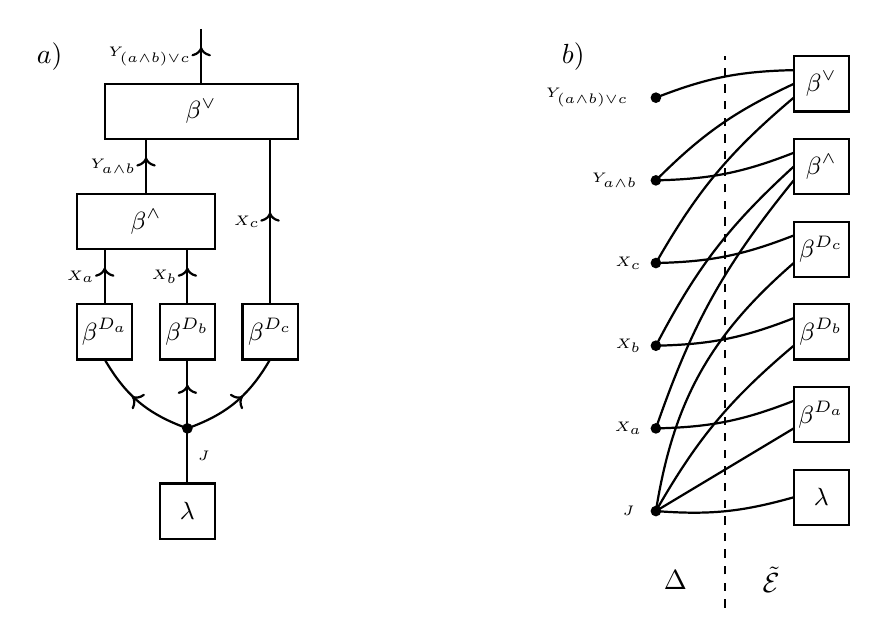
\begin{tikzpicture}[scale=0.35, thick] % , baseline = -3.5pt


    \begin{scope}
        [shift={(23,0)}]

        \node[anchor=center] (text) at (-6,8) {$b)$};

        \draw (2,8) rectangle (4,6);
        \node[anchor=center] (text) at (3,7) {\corelabelsize $\bencodingof{\lor}$};

        \draw (2,5) rectangle (4,3);
        \node[anchor=center] (text) at (3,4) {\corelabelsize $\bencodingof{\land}$};

        \draw (2,2) rectangle (4,0);
        \node[anchor=center] (text) at (3,1) {\corelabelsize $\datacoreof{c}$};

        \draw (2,-1) rectangle (4,-3);
        \node[anchor=center] (text) at (3,-2) {\corelabelsize $\datacoreof{b}$};

        \draw (2,-4) rectangle (4,-6);
        \node[anchor=center] (text) at (3,-5) {\corelabelsize $\datacoreof{a}$};

        \draw (2,-7) rectangle (4,-9);
        \node[anchor=center] (text) at (3,-8) {\corelabelsize $\lambda$};


        \draw[fill] (-3,-8.5) circle (\dotsize);
        \node[anchor=center] (text) at (-4,-8.5) {\colorlabelsize $\indexset$};

        \draw[] (-3,-8.5) to[bend left=-10]  (2,-8);
        \draw[] (-3,-8.5) to[bend left=0]  (2,-5.5);
        \draw[] (-3,-8.5) to[bend left=10]  (2,-2.5);
        \draw[] (-3,-8.5) to[bend left=20]  (2,0.5);


        \draw[fill] (-3,-5.5) circle (\dotsize);
        \node[anchor=center] (text) at (-4,-5.5) {\colorlabelsize $\catvariableof{a}$};

        \draw[] (-3,-5.5) to[bend left=-10]  (2,-4.5);
        \draw[] (-3,-5.5) to[bend left=10]  (2,3.5);

        \draw[fill] (-3,-2.5) circle (\dotsize);
        \node[anchor=center] (text) at (-4,-2.5) {\colorlabelsize $\catvariableof{b}$};

        \draw[] (-3,-2.5) to[bend left=-10]  (2,-1.5);
        \draw[] (-3,-2.5) to[bend left=10]  (2,4);

        \draw[fill] (-3,0.5) circle (\dotsize);
        \node[anchor=center] (text) at (-4,0.5) {\colorlabelsize $\catvariableof{c}$};

        \draw[] (-3,0.5) to[bend left=-10]  (2,1.5);
        \draw[] (-3,0.5) to[bend left=10]  (2,6.5);

        \draw[fill] (-3,3.5) circle (\dotsize);
        \node[anchor=center] (text) at (-4.5,3.5) {\colorlabelsize $\headvariableof{a\land b}$};

        \draw[] (-3,3.5) to[bend left=-10]  (2,4.5);
        \draw[] (-3,3.5) to[bend left=10]  (2,7);

        \draw[fill] (-3,6.5) circle (\dotsize);
        \node[anchor=center] (text) at (-5.5,6.5) {\colorlabelsize $\headvariableof{(a\land b)\lor c}$};

        \draw[] (-3,6.5) to[bend left=10]  (2,7.5);


        \draw[dashed] (-0.5,-12) -- (-0.5,8);

        \node[right] (text) at (0.5,-11) {$\tilde{\edges}$};
        \node[left] (text) at (-1.5,-11) {$\Delta$};

    \end{scope}


    \node[anchor=center] (text) at (-2,8) {$a)$};

    \newcommand{\conposseldec}{3,-5.5}

    \draw[fill] (\conposseldec) circle (\dotsize);
    \draw (\conposseldec) -- (3,-7.5) node[midway, right] {\colorlabelsize ${\indexset}$}; % Unclear, whether this is the best notation!
    \draw[] (2,-7.5) rectangle (4, -9.5);
    \node[anchor=center] (text) at (3,-8.5) {\corelabelsize $\lambda$};

    \draw[-<-] (0,1) -- (0,-1) node[midway,left] {\colorlabelsize $\catvariableof{a}$};
    \draw (-1,-1) rectangle (1, -3);
    \node[anchor=center] (text) at (0,-2) {\corelabelsize $\datacoreof{a}$};
    \draw[-<-] (0,-3) to[bend right=20] (\conposseldec);


    \draw[-<-] (3,1) -- (3,-1) node[midway,left] {\colorlabelsize $\catvariableof{b}$};
    \draw (2,-1) rectangle (4, -3);
    \node[anchor=center] (text) at (3,-2) {\corelabelsize $\datacoreof{b}$};
    \draw[-<-] (3,-3) to[bend right=0]  (\conposseldec);


    \draw[-<-] (6,5) -- (6,-1) node[midway,left] {\colorlabelsize $\catvariableof{c}$};
    \draw (5,-1) rectangle (7, -3);
    \node[anchor=center] (text) at (6,-2) {\corelabelsize $\datacoreof{c}$};
    \draw[-<-] (6,-3) to[bend left=20]  (\conposseldec);


    \draw[-<-] (1.5,5) -- (1.5,3) node[midway,left] {\colorlabelsize $\headvariableof{a \land b}$};
    \draw (-1,3) rectangle (4, 1);
    \node[anchor=center] (text) at (1.5,2) {\corelabelsize $\bencodingof{\land}$};


    \draw[-<-] (3.5,9) -- (3.5,7) node[midway,left] {\colorlabelsize $\headvariableof{(a \land b) \lor c }$};
    \draw (0,7) rectangle (7, 5);
    \node[anchor=center] (text) at (3.5,6) {\corelabelsize $\bencodingof{\lor}$};

\end{tikzpicture}
    \end{center}
    \caption{Example of a Bethe Cluster Graph.
    a) Example of a Tensor Network $\tnetof{\graph}$, which represents the by $\lambda$ averaged evaluation of the formula $(a\land b)\lor c$ on data $\datamap$.
    b) Corresponding Bethe Cluster Hypergraph, which dual is bipartite by the sets $\Delta$ and $\tilde{\edges}$.
    }
    \label{fig:betheDataExample}
\end{figure}

\subsection{Coarse graining}

\begin{definition}
    Let $\graph=(\nodes,\edges)$ and $\secgraph=(\node,\secedges)$ be two hypergraphs sharing their node set and $c: \edges \rightarrow \secedges$ a map.
    We say that $c$ is a coarse graining map and $\secgraph$, if for all $\edgein$
    \begin{align*}
        \edge \subset c(\edge) \, .
    \end{align*}
    For any tensor network $\graphtnetwith$ on $\graph$ we further define a coarse grained tensor network $\sectnetofat{\secgraph}{\nodevariables}$ on $\secgraph$ with hypercores to $\secedge\in\secedges$ by
    \begin{align*}
        \sechypercoreofat{\secedge}{\catvariableof{\secedge}}
        = \contractionof{\{\edgehypercorewith\wcols\secedge=c(\edge)\}}{\catvariableof{\secedge}} \, .
    \end{align*}
\end{definition}

In the literature such coarse graining procedures appear as Cluster Graphs.

We notice that coarse graining of tensor networks preserves their contractions, since
\begin{align*}
    \graphtnetwith
    &= \contractionof{\{\edgehypercorewith\wcols\edgein\}}{\nodevariables} \\
    &= \contractionof{\bigcup_{\secedge\in\secedges}\{\edgehypercorewith\wcols c(\edge)=\secedge\}}{\nodevariables} \\
    &= \contractionof{\{\contractionof{\{\edgehypercorewith\wcols c(\edge)=\secedge\}}{\edgevariables}\wcols\secedge\in\secedges\}}{\nodevariables} \\
    &= \contractionof{\{\sechypercoreofat{\secedge}{\catvariableof{\secedge}}\wcols\secedge\in\secedges\}}{\nodevariables} \\
    &= \sectnetofat{\secgraph}{\nodevariables} \, .
\end{align*}

\subsection{Coarse graining to Tree Hypergraphs}

Construction of coarse grained tree hypergraphs, by the junction tree algorithm
\begin{itemize}
    \item Amounts to triangulation of underlying "extended graph" (i.e. node pairs contained in hypergraphs)
    \item Use the cliques of the triangulated graph as hyperedges (guaranteed to be a tree, a so called "clique tree").
\end{itemize}

\subsubsection{Junction Tree Algorithm}

Classically the junction tree algorithm is formulated on the extended graph (we define extended graphs here by two nodes adjacent if and only if they are contained in a hypergraph) \cite{lauritzen_local_1988}, where one exploits that a graph has a junction tree if and only if it is triangulated \cite{lauritzen_graphical_1996}.
The junction tree algorithm therefore constructs a triangulation of the graph by adding edges (also called chordal graph \cite{koller_probabilistic_2009}), and gets a tree-hypergraph by its cliques.
Note that finding a minimal triangulation is $\mathrm{NP}$-hard.

% Formulation on hypergraphs
We can equally formulate the junction tree algorithm on hypergraphs.
Equivalent to searching for a triangulation of an extended graph, we here search for a coarse grained hypergraph, which is a tree.
Then the cliques of the triangulated graphs correspond with the hyperedges of the coarse grained hypergraph.

\red{Triangulation via Delta transform:
Choice of delta tensors and assignment to hyperedges amounts to triangulation procedure (i.e. combination of Bethe transform and coarse graining).
}

\subsubsection{Variable Elimination}

\red{Needs Delta tensor assignments at each elimination step!}

Based on disjoint subsets of $\nodes$ we can construct a coarse graining procedure of a hypergraph:
Construct iteratively $\secedges$ by iterating through the node subsets and
\begin{itemize}
    \item Add those $\edge\in\edges$ which have not been assigned before and contain variables in the subset.
    \item Choose the new edge by the union of the old one with the assigned edges in $\edges$ and dropping those nodes, which are not appearing in the rest of $\edges$ any more.
    \item Return the intersection of the new edge with the rest of $\edges$ back to $\edges$.
\end{itemize}
By construction this gives a tree hypergraph.

    \section{Boolean Propagation}\label{sec:booleanPropagation}

\red{Sound in the sense that entailment decisions made during the propagation are always true.}

Instead of the exact calculation of a contraction, let us now investigate schemes to sparsify the tensors before a contraction.
To this end, we first show underlying properties of contractions enabling these schemes.

To state the next theorem we use the nonzero function $\nonzerofunction: \rr \rightarrow [2]$ by $\nonzeroof{x}=1$ if $x\neq0$ and $\nonzeroof{x}=0$ else.
Applied coordinatewise on tensors $\hypercorewith$ it marks the nonzero coordinates by $1$.
The resulting boolean tensor is denoted by $\nonzeroof{\hypercorewith}$.

Further, we use the partial order $\prec$ of boolean tensors, which is defined by
\begin{align*}
    \hypercoreat{\shortcatvariables} \prec \sechypercoreat{\shortcatvariables}
    \quad \Leftrightarrow \quad
    \uniquantwrtof{\shortcatindicesin}{\hypercoreat{\indexedshortcatvariables}\leq\sechypercoreat{\indexedshortcatvariables} }
\end{align*}
%We use the coordinatewise nonzero indicator $\nonzeroof{\cdot}$, which returns a boolean tensor indicating which coordinates of $\hypercorewith$ vanish.

\begin{theorem}
    \label{the:mpGuaranteeBoolean}
    For any implementation of \algoref{alg:contractionPropagation} we have at any stage of the algorithm for any message channel $(\sedge,\redge)$
    \begin{align*}
        \nonzeroof{\contractionof{\extnetwith}{\catvariableof{\sedge\cap\redge}}}
        \prec\nonzeroof{\messagewith} \, .
    \end{align*}
\end{theorem}

To show this theorem we in the following proof the monotonicity of tensor contractions and the invariance of adding supports of subcontractions.

\subsection{Monotonicity of Tensor Contraction}

We show that adding boolean tensor cores to a contraction orders the results by the partial ordering introduced in \defref{def:partialOrder}.

\begin{theorem}[Monotonicity of Tensor Contractions]
    \label{the:monotonicityBinaryContractions}
    Let $\extnet, \secextnet$ be tensor network of non-negative tensors and $\catvariableof{\secnodes}$ an arbitrary set of random variables. %, and $\tilde{\theta}$ another binary tensor.
    Then we have
    \begin{align*}
        \nonzeroof{\contractionof{\extnet\cup\secextnet}{\catvariableof{\secnodes}}} \prec
        \nonzeroof{\contractionof{\extnet}{\catvariableof{\secnodes}}} \, .
    \end{align*}
\end{theorem}
\begin{proof}
    It suffices to show that for any $\catindexof{\secnodes}$ with
    \[ \nonzeroof{\contractionof{\extnet\cup\secextnet}{\indexedcatvariableof{\secnodes}}}=1 \]
    we also have
    \[ \nonzeroof{\contractionof{\extnet}{\indexedcatvariableof{\secnodes}}}=1 \, . \]
    For any $\catindexof{\secnodes}$ satisfying the first equation we find an extension $\catindexof{\nodes}$ to all variables of the tensor networks such that
    \[ \contractionof{\extnet\cup\secextnet}{\indexedcatvariableof{\nodes}} > 0 \]
    and it follows that
    \[ \contractionof{\extnet}{\indexedcatvariableof{\nodes}} > 0 \andspace  \contractionof{\secextnet}{\indexedcatvariableof{\nodes}} > 0  \, . \]
    But this already implies, that
    \begin{align*}
        \nonzeroof{\contractionof{\extnet}{\indexedcatvariableof{\secnodes}}}=1 \, . & \qedhere
    \end{align*}
\end{proof}


\begin{lemma}
    \label{lem:monotonocityPreservedUnderContractions}
    Let $\extnet$ and $\secextnet$ be non-negative tensor networks on the same hypergraph, and let us assume that for all $\edgein$
    \begin{align*}
        \nonzeroof{\hypercoreofat{\edge}{\catvariableof{\edge}}}
        \prec \nonzeroof{\sechypercoreofat{\edge}{\catvariableof{\edge}}} \, .
    \end{align*}
    Then we have for any subset $\secnodes$ %! If for smaller subsets need to demand non-negativity!
    \begin{align*}
        \nonzeroof{\contractionof{\extnet}{\catvariableof{\secnodes}}}
        \prec \nonzeroof{\contractionof{\secextnet}{\catvariableof{\secnodes}}} \, .
    \end{align*}
\end{lemma}
\begin{proof}
    It is sufficient to show that for all $\seccatindexof{\secnodes}\in\bigtimes_{\node\in\secnodes}[\catdimof{\node}]$ we have
    \begin{align*}
        \left(\nonzeroof{\contractionof{\extnet}{\catvariableof{\secnodes}=\seccatindexof{\secnodes}}}=1\right)
        \Rightarrow
        \left(\nonzeroof{\contractionof{\secextnet}{\catvariableof{\secnodes}=\seccatindexof{\secnodes}}}=1\right) \, .
    \end{align*}
    If and only if for there is an index $\catindexof{\nodes}$ with $\restrictionofto{\catindexof{\nodes}}{\secnodes}=\seccatindexof{\secnodes}$ with
    \begin{align*}
        \uniquantwrtof{\edgein}{
            \hypercoreofat{\edge}{\indexedcatvariableof{\edge}}=1
        }
    \end{align*}
    then $\nonzeroof{\contractionof{\extnet}{\catvariableof{\secnodes}=\seccatindexof{\secnodes}}}=1$.
    Note, that by assumption we have for this index also
    \begin{align*}
        \uniquantwrtof{\edgein}{
            \sechypercoreofat{\edge}{\indexedcatvariableof{\edge}}=1
        }
    \end{align*}
    and thus $\nonzeroof{\contractionof{\secextnet}{\catvariableof{\secnodes}=\seccatindexof{\secnodes}}}=1$.
\end{proof}

\subsection{Invariance of Adding Subcontractions}

%We now show \theref{the:booleanContractionInvariance} of \charef{cha:logicalReasoning}.
Let us now state an equivalence of the contraction, when we add the result of the same contraction.
This property was used in the proof of \theref{the:soundnessKnowledgePropagation}.

\begin{theorem}[Invariance under adding subcontractions]
    \label{the:invarianceAddingSubcontractions}
    Let $\extnet$ be a tensor network of non-negative tensors with variables $\catvariableof{\nodes}$ and let $\secextnet$ be a subset.
    Then we have for any subset $\catvariableof{\secnodes}$ of $\catvariableof{\nodes}$
    \begin{align*}
        \contractionof{\extnet \cup\left\{
            \nonzeroof{
                \contractionof{\secextnet}{\catvariableof{\secnodes}}
            }
            \right\}}{\catvariableof{\nodes}}
        = \contractionof{\extnet}{\catvariableof{\nodes}}
        \, .
    \end{align*}
\end{theorem}
\begin{proof}
    For any $\catindexof{\nodes}$ with
    \[ \contractionof{\extnet}{\indexedcatvariableof{\nodes}} = 0 \]
    we also have
    \[ \contractionof{\extnet \cup\{
        \nonzeroof{
            \contractionof{\secextnet}{\catvariableof{\secnodes}}
        }
        \}}{\indexedcatvariableof{\nodes}} = 0 \, . \]
    For any $\catindexof{\nodes}$ with
    \[ \contractionof{\extnet}{\indexedcatvariableof{\nodes}} \neq 0 \]
    we have for the reduction $\catindexof{\secnodes}$ of the index $\catindexof{\nodes}$ that
    \[  \contractionof{\secextnet}{\indexedcatvariableof{\secnodes}} \neq 0 \]
    and thus
    \begin{align*}
        \contractionof{\extnet \cup\{
            \nonzeroof{
                \contractionof{\secextnet}{\catvariableof{\secnodes}}
            }
            \}}{\indexedcatvariableof{\nodes}}
        &= \contractionof{\extnet}{\indexedcatvariableof{\nodes}} \cdot \nonzeroof{
            \contractionof{\secextnet}{\catvariableof{\secnodes}}
        }[\indexedcatvariableof{\secnodes}] \\
        &= \contractionof{\extnet}{\indexedcatvariableof{\nodes}} \, . \qedhere
    \end{align*}
%	When the subcore transformed by $\nonzeroof{\cdot}$ contains a zero slice, then this
%	 zero slice is also appearing in the rest contraction.
%	Multiplying a zero slice with zero does not affect the contraction, neither does multiplication with one on any slice.
\end{proof}

\subsection{Consequences for boolean Contraction Propagation}

\begin{lemma}
    \label{lem:messageMonotonicity}
    In any implementation of \algoref{alg:contractionPropagation} and at any iteration of the $\mathrm{While}$ loop, we have the old message $\mesfromtowith{\secsedge}{\redge}$ and the updated message $\updatedmesfromtowith{\secsedge}{\redge}$ obey
    \begin{align*}
        \mesfromtowith{\secsedge}{\redge} \prec \updatedmesfromtowith{\secsedge}{\redge} \, .
    \end{align*}
\end{lemma}
\begin{proof}
    By induction over the iterations of the $\mathrm{While}$ loop, and using monotonicity of contractions. % Would help to state this for
\end{proof}

We are now ready to show the above guarantee on the soundness of message passing.

\begin{proof}[Proof of \theref{the:mpGuaranteeBoolean}]
    We first show via induction on the message updates that at any stage of \algoref{alg:contractionPropagation} we have
    \begin{align}
        \label{eq:contractionWithMessageSupport}
        \contraction{\tnetofat{\graph}{\nodevariables}}{\nodevariables}
        = \contractionof{\tnetofat{\graph}{\nodevariables} \cup \{\nonzeroof{\messagewith} \wcols (\sedge,\redge) \in \dirovgraph\}}{\nodevariables} \, .
    \end{align}
    Since the messages are initialized by trivial tensors, this is true after the initialization of \algoref{alg:contractionPropagation}.
    Now we assume that this equation holds at an arbitrary state of the algorithm at the start of the $\mathrm{While}$ loop, and let $(\sedge,\redge)$ be the channel chosen by the scheduler.
    Then we choose
    \begin{align*}
        \secextnet = \{\hypercoreofat{\sedge}{\redge} \}
        \cup \{\mesfromtowith{\secsedge}{\sedge} \wcols (\secsedge,\sedge) \in \dirovgraph \ncond \secsedge\neq\redge\}
    \end{align*}
    and apply \theref{the:invarianceAddingSubcontractions} to get
    \begin{align*}
        \contraction{\tnetofat{\graph}{\nodevariables}}{\nodevariables}
        &=\contractionof{\tnetofat{\graph}{\nodevariables} \cup \{\nonzeroof{\mesfromtowith{\thirdsedge}{\secsedge}} \wcols (\thirdsedge,\secsedge) \in \dirovgraph\}}{\nodevariables} \\
        &= \contractionof{\tnetofat{\graph}{\nodevariables} \cup \{\nonzeroof{\mesfromtowith{\thirdsedge}{\secsedge}} \wcols (\thirdsedge,\secsedge) \in \dirovgraph\}
            \cup \{\nonzeroof{
                \contractionof{
                    \secextnet
                }{\catvariableof{\sedge\cap\redge}}
            }\}
        }{\nodevariables} \\
%    \end{align*}
%    We notice that the inner contraction is just the support of the updated message
%    \begin{align*}
%        \contraction{\tnetofat{\graph}{\nodevariables}}{\nodevariables}
        &= \breakablecontractionof{\tnetofat{\graph}{\nodevariables}
        \cup \{\nonzeroof{\mesfromtowith{\thirdsedge}{\secsedge}} \wcols (\thirdsedge,\secsedge)  \in \dirovgraph \ncond (\thirdsedge,\secsedge)\neq(\sedge,\redge) \} \\
        & \quad\quad\quad\quad \cup \{\nonzeroof{\mesfromtowith{\sedge}{\redge}},\nonzeroof{\updatedmesfromtowith{\sedge}{\redge}}\}
        }{\nodevariables} \\
        & = \breakablecontractionof{\tnetofat{\graph}{\nodevariables}
        \cup \{\nonzeroof{\mesfromtowith{\thirdsedge}{\secsedge}} \wcols (\thirdsedge,\secsedge)  \in \dirovgraph \ncond (\thirdsedge,\secsedge)\neq(\sedge,\redge) \} \\
        & \quad\quad\quad\quad \cup \{\nonzeroof{\updatedmesfromtowith{\sedge}{\redge}}\}
        }{\nodevariables} \, .
    \end{align*}
    Here we used that by \lemref{lem:messageMonotonicity} we have
    \begin{align*}
        \contractionof{\nonzeroof{\mesfromtowith{\sedge}{\redge}},\nonzeroof{\updatedmesfromtowith{\sedge}{\redge}}}{\catvariableof{\sedge\cap\redge}}
        = \nonzeroof{\updatedmesfromtowith{\sedge}{\redge}} \, .
    \end{align*}
    We therefore have by induction \eqref{eq:contractionWithMessageSupport} during the algorithm.

    The claim now follows from \theref{the:monotonicityBinaryContractions}, since
    \begin{align*}
        &\nonzeroof{\contractionof{\tnetofat{\graph}{\nodevariables} \cup \{\nonzeroof{\messagewith} \wcols (\sedge,\redge) \in \dirovgraph\}}{\catvariableof{\sedge\cap\redge}}} \\
        &\quad\quad \prec \nonzeroof{\nonzeroof{\messagewith}} = \nonzeroof{\messagewith} \, . &\qedhere
    \end{align*}
\end{proof}


\section{Complete Unit Clause Propagation (UCP)}

\red{Investigate here three conditions, where constraint propagation is also complete. (tree condition holds more general!)}

Unit clauses are assignments to single variables.
They are propagated between clusters of formulas

UCP is \algoref{alg:contractionPropagation} in case of bethe hypergraphs (having bipartite overlap graphs with nodes to previous hyperedges and variable nodes), and using the constraint propagation implementation, that is
%UCP is Knowledge Propagation (see Algorithm~1 in the report) in case of
\begin{itemize}
    \item Hypergraph with hyperedges to single variables and to previous edges
%    \item Domain edges by single variable nodes, i.e.
%    \begin{align*}
%        \domainedges = \big\{\{\node\}\wcols\nodein\big\}
%    \end{align*}
    \item Initial queue by those edges containing single nodes
    \begin{align*}
        \graphqueue = \big\{\{\node\}\wcols\{\node\}\in\edges\big\}
    \end{align*}
\end{itemize}
After termination of the Knowledge Propagation Algorithm we return $"UNSAT"$, if any knowledge core vanishes.
In that case we have an unsatisfiable CSP.
If no knowledge core vanishes, we define $\variableset$ as the subset of variables with nontrivial knowledge cores and output $\catindex_{\variableset}$ where for $\node\in\variableset$
%    extract from the nontrivial Knowledge cores (labeled by $\variableset$) an assignment
\begin{align*}
    \catindex_{\node} = \invonehotmapof{\kcoreat{\{\node\}}} \, .
\end{align*}

We always have, that UCP is sound (since KP is sound).

\begin{definition}
    We say that UCP is complete for a CSP, if it outputs $"UNSAT"$ or for no node $\node\in\variableset$ we have that at all solutions of the CSP have the same index at $\node$.
\end{definition}

\subsection{Forward Chaining for Horn-SAT}

\begin{definition}[Definite Horn-SAT]
    Let $\extnetasset$ be a CSP.
    We say it is a definite Horn-SAT problem, if each $\hypercoreof{\edge}$ is a clause, which has exactly one positive literal.
\end{definition}

Forward chaining is a linear time and complete satisfiability checker on Horn Logic (a subset of Propositional Logic where each clause has at most one positive literal).
\begin{itemize}
    \item Messages passed are the one-hot encodings of assignment to single variables (unit clauses).
    \item Clusters are the Horn clauses, which receive messages for their negative literals.
    A Cluster sends a nontrivial message to a variable, if the variable is the only unassigned literal in the clause and the clause has not been satisfied yet.
\end{itemize}

\begin{lemma}
    Let $\extnet=\extnetasset$ be a Definite Horn-SAT problem, then UCP does never output $"UNSAT"$.
    Let further $\catindexof{\variableset}$ be the output of UCP.
    Then $\catindexof{\node}=1$ for each $\node\in\variableset$ and
    \begin{align*}
        1_{\variableset} \times 0_{\nodes/\variableset} \quad \text{and} \quad 1_{\variableset} \times 1_{\nodes/\variableset}
    \end{align*}
    are solutions of $\extnet$.
\end{lemma}
\begin{proof}
    First of all, when all knowledge cores are trivial, vanishing or $\tbasis$, then the nonzero transformation of any contraction is trivial, vanishing or $\tbasis$.
    Thus, since this assumption is met at the start all knowledge cores remain such during the algorithm.

    At the termination of UCP we simplify the definite clauses by erasing the literals in $\variableset$.
    This erasure results either in empty clauses or in definite clauses with at least $2$ literals, since otherwise the algorithm would not have terminated.
    Since at least one positive and one negative literal remain, these are satisfied if all atoms are $1$ and if all atoms are $0$.
\end{proof}


\begin{theorem}
    UCP for Definite Horn-SAT is complete.
\end{theorem}
\begin{proof}
    From the above lemma we know that the remaining variables are in at least one solution $0$ and in at least one $1$.
    Thus they are neither entailed nor contradicted.
\end{proof}

\subsection{UCP for 2-SAT}

\begin{definition}[2-SAT]
    Let $\extnetasset$ be a CSP.
    We say it is an 2-SAT problem, if each $\hypercoreof{\edge}$ has order at most 2 and is a clause.
\end{definition}

%Each $\hypercoreof{\edge}$ in a 2-SAT problem is by definition a clause of at most two literals.

2-SAT is in P and can be solved by the message passing algorithm Unit Clause Propagation (UCP).
\begin{itemize}
    \item At each connected component of the problems factor graph, choose on variable an do the message passing scheme below with initialization by the variable on $0$ and on $1$.
    \item Messages passed are the one-hot encodings of assignment to single variables (unit clauses).
    \item Any clause that receives a message has only a single literal left and either gets directly trivial (if the message coincides with the literal) or assigns the remaining variable and passes further.
\end{itemize}

\begin{lemma}
    Let $\extnetasset$ be a 2-SAT instance.
    Given the outputs $\catindex_c^{s_c}$, $s_c\in [n_c]$ and $n_c\in\{0,1,2\}$ of UCP for each connected component $c \subset \nodes$ we have
    \begin{align*}
        \contractionof{\extnetasset}{\nodevariables}
        = \bigotimes_{c} \left( \sum_{s_c\in[n_c]} \onehotmapofat{\catindex_c^{s_c}}{\catvariableof{c}}\right) \, .
    \end{align*}
\end{lemma}
\begin{proof}
    For each component $c$ of $\graph$ we choose a start variable and choose a value $x_\node \in [2]$.
    We then have
    \begin{align*}
        \contractionof{\tnetof{c}\cup\{\onehotmapofat{x_\node}{\catvariableof{\node}}\}}{\catvariableof{c}}
        = \begin{cases}
              \zerosat{\catvariableof{c}} & \text{if UCP returns "UNSAT"} \\
              \onehotmapofat{\catindex_c^{s_c}}{\catvariableof{c}} & \text{if UCP returns $\catindex_c^{s_c}$}
        \end{cases} \, .
    \end{align*}
\end{proof}

We use UCP for entailment/contradiction decision by checking whether for each $\atomenumerator\in c$ $x_\atomenumerator^{s_c}$ is constant.
Exception: When one component is not sat, the whole 2-SAT instance is unsatisfiable and all entailment and contradiction properties hold.

\begin{theorem}
    UCP for 2-SAT is complete.
\end{theorem}
\begin{proof}
    We assume that 2-SAT at hand is satisfiable.
    Exactly when $x_\node^{s_c}$ is constant for $s_c\in[n_c]$ we can write, using the above Lemma
    \begin{align*}
        \contractionof{\extnetasset}{\nodevariables}
        = \onehotmapofat{x_\atomenumerator^{s_c}}{\catvariableof{\atomenumerator}} \otimes
        \contractionof{\extnetasset}{\catvariableof{\nodes/\{\node\}}} \, .
    \end{align*}
    In case of $x_\node^{s_c}=1$ this is an equivalent criterion for entailment (respectively contradiction in case of $x_\node^{s_c}=0$).
\end{proof}

\subsection{UCP for Tree-SAT}

\begin{definition}[Tree-SAT]
    Let $\extnetasset$ be a CSP.
    We say it is an Tree-SAT problem, if the factor graph is minimal connected.
\end{definition}

Note that we do not demand the constraint cores to be clauses in the Tree-SAT definition.

We modify UCP slightly:
If any constraint tensor is decomposed into a tensor product of a basis vector of one variable and an arbitrary rest tensor, the constraint tensor is added to the queue at initialization.

\begin{theorem}
    The modified UCP for Tree-SAT is complete.
\end{theorem}
\begin{proof}
    Since the message-passing provides exact contractions and the messages in UCP communicate the support.
\end{proof}


\subsection{Outlook}

\subsubsection{With backtracking: DPLL for generic SAT}

DPLL combines backtracking search with unit clause propagation (UCP).
A form of message passing is applied to reduce the clauses given the current partial assignment:
When guessed an assignment to a variable, the variable is removed from all clauses, either making the clause trivial (coinciding assignment) or smaller.
If only one literal remains in a clause, the variable would be assigned accordingly (unit propagation).
This can be directly done in the intermediate message passing scheme, or understood as the next backtracking step ("Find-Unit-Clause" in Figure 7.17 in \cite{russell_artificial_2021}).

\subsubsection{With randomization: WalkSAT}

WalkSAT is a stochastic local search algorithm for SAT.
It starts with a random assignment and iteratively flips variables to reduce the number of unsatisfied clauses.
This can be understood as a (modified) Gibbs sampling algorithm, where the number of unsatisfied clauses is the energy function to be minimized.
The modifications are:
\begin{itemize}
    \item Selection of variable to be resampled: Typically chosen by looking at unsatisfied clauses and picking a variable that minimizes the number of newly unsatisfied clauses (whereas in Gibbs sampling one follows a fixed variable order).
    \item Marginal probability: Typically fixed by a mixing parameter, whereas in Gibbs sampling would be sensitive to the energy differences.
\end{itemize}


    \section{Basis Propagation}\label{sec:basisPropagation}

\begin{theorem}
    \label{the:mpGuaranteeBasis}
    Given a directed acyclic hypergraph and a tensor network of directed boolean tensors respecting the hypergraph.
    Then the final messages of \algoref{alg:contractionPropagation} in the directed implementation are exact.
\end{theorem}
\begin{proof}
    Just show inductively that the messages are one-hot encodings of the function evaluation.
\end{proof}

%% Basis calculus interpretation
We have an interpretation of the messages by one-hot encodings of function evaluation at each node.
The basis vectors at the leafs (i.e. edges with no incoming nodes) are understood as one-hot encodings of inputs.
Passing a message $\onehotmapof{i}$ in direction thus gives the message $\onehotmapof{\exfunction(i)}$.

%% Acyclicity
Note, that the assumptions of \theref{the:mpGuaranteeBasis} are met, whenever the graph is directed and acyclic.
We do not need acyclicity of the underlying undirected graph.

%% Needed? -> just basis calculus. SVD Perspective
This is because any basis encoding of a function, the decomposition
\begin{align*}
    \bencodingof{\exfunction} = \sum_{y \in\imageof{\exfunction}} ( \sum_{i: \exfunction(i)=y}\onehotmapof{i} )  \otimes \onehotmapof{y}
\end{align*}
is a SVD of the matrification of $\bencodingof{\exfunction}$ with respect to incoming and outgoing legs.

%\red{Interpretation as dataset evaluation.}

\begin{example}[Function evaluation on a dataset]
    Let the only non-basis vectors be the incoming ones, e.g. by a dataset (i.e. averaging by $\onesat{\decvariable}$).
    Message Passing of directed and boolean message by basis encoding of functions can be interpreted as function evaluation.
    Each subfunction evaluation is passed in its one-hot encoding.
    Distinguish:
    \begin{itemize}
        \item Single inference: Basis propagation (see \figref{fig:basPropDatapoint})
        \item Batchwise inference: "Tensor Parallelism", but in the most interesting cases not exact.
        If the graph is minimally connected, we are guaranteed that the averages are exact.
        Also we can apply boolean theory to have sound messages: If in a message a state is not supported, this state cannot be reached by any data point
    \end{itemize}

    \begin{figure}
        \begin{center}
            \newcommand{\basispropdatasketchdrawat}[2]{
\begin{scope}[shift={(#1,#2)}]
    \newcommand{\conposseldec}{5,-5.5}
    \draw[fill] (\conposseldec) circle (\dotsize);
    \draw (\conposseldec) -- (5,-7) node[midway, right] {\colorlabelsize ${\indexset}$}; % Unclear, whether this is the best notation!
    \draw[] (4,-7) rectangle (6, -9);
    \node[anchor=center] (text) at (5,-8) {\corelabelsize $\onehotmapof{\datindex}$};

    \draw[-<-] (0,1) -- (0,-1) node[midway,left] {\colorlabelsize $\catvariableof{a}$};
    \draw (-1,-1) rectangle (1, -3);
    \node[anchor=center] (text) at (0,-2) {\corelabelsize $\datacoreof{a}$};
    \draw[-<-] (0,-3) to[bend right=20] (\conposseldec);

    \draw[-<-] (7,1) to[bend right=-15] (5,-1) ;
    \draw[-<-] (3,1) to[bend right=15] (5,-1) ;
    \draw[-<-] (5,-1) -- (5,-2)node[midway,left] {\colorlabelsize $\catvariableof{b}$};
    \drawvariabledot{5}{-1}
    \draw (4,-2) rectangle (6, -4);
    \node[anchor=center] (text) at (5,-3) {\corelabelsize $\datacoreof{b}$};
    \draw[-<-] (5,-4) to[bend right=0]  (\conposseldec);

    \draw (9,-1) rectangle (11, -3);
    \node[anchor=center] (text) at (10,-2) {\corelabelsize $\datacoreof{c}$};
    \draw[-<-] (10,-3) to[bend left=20]  (\conposseldec);
    \draw[-<-] (10,1) -- (10,-1) node[midway,right] {\colorlabelsize $\catvariableof{c}$};

    \draw[-<-] (1.5,5) -- (1.5,3) node[midway,left] {\colorlabelsize $\headvariableof{a \land b}$};
    \draw (-1,3) rectangle (4, 1);
    \node[anchor=center] (text) at (1.5,2) {\corelabelsize $\bencodingof{\land}$};

    \draw[-<-] (8.5,5) -- (8.5,3) node[midway,left] {\colorlabelsize $\headvariableof{b \Rightarrow c}$};
    \draw (6,3) rectangle (11, 1);
    \node[anchor=center] (text) at (8.5,2) {\corelabelsize $\bencodingof{\Rightarrow}$};

    \draw[-<-] (5,9) -- (5,7) node[midway,left] {\colorlabelsize $\headvariableof{(a \land b) \lor (b \Rightarrow c) }$};
    \draw (0,7) rectangle (10, 5);
    \node[anchor=center] (text) at (5,6) {\corelabelsize $\bencodingof{\lor}$};
\end{scope}
}


\begin{tikzpicture}[scale=0.3, thick] % , baseline = -3.5pt


    \basispropdatasketchdrawat{0}{0}
    \node[anchor=center] at  (-2,6.5) {\corelabelsize $1)$};
    \draw[\newmessagecolor,dashed,->] (3,-8) to [bend right=-30] (0,-4);
    \node[anchor=center,\newmessagecolor] at (1,-7.5) {\corelabelsize $\onehotmapof{\datindex}$};

    \draw[\newmessagecolor,dashed,->] (7,-8) to [bend right=30] (10,-4);
    \node[anchor=center,\newmessagecolor] at (9,-7.5) {\corelabelsize $\onehotmapof{\datindex}$};

    \draw[\newmessagecolor,dashed,->] (6.5,-6.5) to [bend right=50] (6.5,-3); % node[right] {\corelabelsize $\onehotmapof{\datindex}$};
    \node[anchor=center,\newmessagecolor] at (7.75,-3) {\corelabelsize $\onehotmapof{\datindex}$};

    \basispropdatasketchdrawat{18}{0}
    \begin{scope}[shift={(18,0)}]
        \node[anchor=center] at  (-2,6.5) {\corelabelsize $2)$};
        \draw[\oldmessagecolor,dashed,->] (3,-8) to [bend right=-30] (0,-4);
        \node[anchor=center,\oldmessagecolor] at (1,-7.5) {\corelabelsize $\onehotmapof{\datindex}$};

        \draw[\oldmessagecolor,dashed,->] (7,-8) to [bend right=30] (10,-4);
        \node[anchor=center,\oldmessagecolor] at (9,-7.5) {\corelabelsize $\onehotmapof{\datindex}$};

        \draw[\oldmessagecolor,dashed,->] (6.5,-6.5) to [bend right=50] (6.5,-3);
        \node[anchor=center,\oldmessagecolor] at (7.75,-3) {\corelabelsize $\onehotmapof{\datindex}$};

        \draw[\newmessagecolor,dashed,->] (6.5,-2.5) to [bend right=20] (7.75,0.5);
        \node[anchor=center,\newmessagecolor] at (9,-0.25) {\corelabelsize $\onehotmapof{b^\datindex}$};

        \draw[\newmessagecolor,dashed,->] (3.5,-2.5) to [bend right=-20] (2.25,0.5);
        \node[anchor=center,\newmessagecolor] at (1.25,-0.25) {\corelabelsize $\onehotmapof{b^\datindex}$};

        \draw[\newmessagecolor,dashed,->] (11.5,-2) to [bend right=50] (11.5,1);
        \node[anchor=center,\newmessagecolor] at (13,-0.5) {\corelabelsize $\onehotmapof{c^\datindex}$};

        \draw[\newmessagecolor,dashed,->] (-1.5,-2) to [bend right=-50] (-1.5,1);
        \node[anchor=center,\newmessagecolor] at (-3,-0.5) {\corelabelsize $\onehotmapof{a^\datindex}$};

    \end{scope}

    \basispropdatasketchdrawat{36}{0}
    \begin{scope}[shift={(36,0)}]
            \node[anchor=center] at  (-2,6.5) {\corelabelsize $3)$};
%        \draw[\oldmessagecolor,dashed,->] (3,-8) to [bend right=-30] (0,-4);
%        \node[anchor=center,\oldmessagecolor] at (1,-7.5) {\corelabelsize $\onehotmapof{\datindex}$};
%
%        \draw[\oldmessagecolor,dashed,->] (7,-8) to [bend right=30] (10,-4);
%        \node[anchor=center,\oldmessagecolor] at (9,-7.5) {\corelabelsize $\onehotmapof{\datindex}$};
%
%        \draw[\oldmessagecolor,dashed,->] (6.5,-6.5) to [bend right=50] (6.5,-3);
%        \node[anchor=center,\oldmessagecolor] at (7.75,-3) {\corelabelsize $\onehotmapof{\datindex}$};

        \draw[\oldmessagecolor,dashed,->] (6.5,-2.5) to [bend right=20] (7.75,0.5);
        \node[anchor=center,\oldmessagecolor] at (9,-0.25) {\corelabelsize $\onehotmapof{b^\datindex}$};

        \draw[\oldmessagecolor,dashed,->] (3.5,-2.5) to [bend right=-20] (2.25,0.5);
        \node[anchor=center,\oldmessagecolor] at (1.25,-0.25) {\corelabelsize $\onehotmapof{b^\datindex}$};

        \draw[\oldmessagecolor,dashed,->] (11.5,-2) to [bend right=50] (11.5,1);
        \node[anchor=center,\oldmessagecolor] at (13,-0.5) {\corelabelsize $\onehotmapof{c^\datindex}$};

        \draw[\oldmessagecolor,dashed,->] (-1.5,-2) to [bend right=-50] (-1.5,1);
        \node[anchor=center,\oldmessagecolor] at (-3,-0.5) {\corelabelsize $\onehotmapof{a^\datindex}$};

        \draw[\newmessagecolor,dashed,->] (11.5,2) to [bend right=60] (10.5,5);
        \node[anchor=center,\newmessagecolor] at (14,3.5) {\corelabelsize $\onehotmapof{(b\Rightarrow c)^\datindex}$};

        \draw[\newmessagecolor,dashed,->] (-1.5,2) to [bend right=-60] (-0.5,5);
        \node[anchor=center,\newmessagecolor] at (-3.75,3.5) {\corelabelsize $\onehotmapof{(a\land b)^\datindex}$};

    \end{scope}
\end{tikzpicture}

        \end{center}
        \caption{
            Behavior of the contraction propagation algorithm \algoref{alg:contractionPropagation} for the evaluation of the formula $(\catvariableof{a}\land\catvariableof{b})\lor(\catvariableof{b}\Rightarrow\catvariableof{c})$ on a datapoint $(a^{\datindex},b^{\datindex},c^{\datindex})$, which is selected from a dataset $\datamap$.
            The algorithm is executed in the directed implementation, in which each message is sent exactly once.
            We sketch the $9$ iterations of the $\mathrm{While}$ loop until the algorithm terminates in the epochs $1)$ (selection of the datapoint from the dataset) $2)$ (computation of finest formula components) and $3)$  (computation of coarser formula components) .
            In each epoch we sketch in gray the received messages at the previous epoch and in blue the sent messages.
            Since the hypercores are directed and boolean, the messages are one-hot encodings interpreted as evaluations of associated functions.
        }\label{fig:basPropDatapoint}
    \end{figure}

\end{example}
% Tensor Parallelism outlook


%After having established a one-to-one connection between the directed and binary tensors with the encoding of functions, we now interpret contractions as evaluations of the respective functions.
%Applying this insight iteratively on composed functions we show the following theorem.

\begin{remark}[Basis Calculus as Message Passing]
    Given a tensor network of directed and binary tensor cores, each representing a function $\exfunctionof{\edge}$ depending on variables $\incomingnodes$.
    When there are not directed cycles, we define the compositions of $\exfunctionof{\edge}$ to be the function $\exfunction$ from the nodes $\nodesone$ not appearing as incoming nodes to the nodes $\nodestwo$ not appearing as outgoing nodes in an edge.
    Choosing arbitrary $\catindexof{\node}\in[\catdimof{\node}]$ for $\node\in\nodesone$ we have
    \begin{align*}
        \contractionof{\{\bencodingofat{\exfunctionof{\edge}}{\catvariableof{\outgoingnodes},\catvariableof{\incomingnodes}} \, : \edge=(\outgoingnodes,\incomingnodes)\in\edges\}}{\nodestwo}
        = \onehotmapof{\exfunction(\catindexof{\node} \wcols \node\in\nodesone)}\, .
    \end{align*}
\end{remark}



    \section{Generalizations}

There are two generalization directions:
\begin{itemize}
    \item Kikuchi message passing schemes: Messages are sent between layers of hyperedges (where so far have the hyperedges and their intersections in two layers).
    \item Expectation-propagation on generalized features:
    Hyperedges are understood as sets of features.
    Messages are computed by forward map in the whole inference cluster, and backward map in the message cluster.
    So far: Used only the hybrid indicator features on the edges, for which forward maps are simple contractions.
\end{itemize}

    \bibliographystyle{plainnat}
    \bibliography{../../references.bib}


\end{document}